%!TEX root = ../dissertation.tex
\chapter{Line Spectrum Estimation}
\label{chap:linespect}

\section{Introduction}

Extracting the frequencies and relative phases of a superposition of complex
exponentials from a small number of noisy time samples is a foundational problem
in statistical signal processing. These \emph{line spectral estimation} problems
arise in a variety of applications, including the direction of arrival
estimation in radar target identification~\cite{radar}, sensor array signal
processing~\cite{arrays} and imaging systems~\cite{imaging} and also underlies
techniques in ultra wideband channel estimation~\cite{uwb},
spectroscopy~\cite{nmr}, molecular dynamics~\cite{andrade2012}, and power
electronics~\cite{power}


Despite of hundreds of years of research on the fundamental problem of line
spectrum estimation, there still remain several open questions in this area.
This chapter addresses a central one of these problems: how well can we
determine the locations and magnitudes of spectral lines from noisy temporal
samples? We establish lower bounds on how well we can recover such signals and
demonstrate that these worst case bounds can be nearly saturated by solving a
convex programming problem. Moreover, we prove that the estimator approximately
localizes the frequencies of the true spectral lines.

While polynomial interpolation using Prony's technique can estimate the
frequency content of a signal \emph{exactly} from as few as $2k$ samples if
there are $k$ frequencies, Prony's method is inherently unstable due to
sensitivity of polynomial root finding. Several methods have been proposed to
provide more robust polynomial interpolation~\cite{music,esprit,hua02} (for an
extensive bibliography on the subject, see ~\cite{stoica93}), and these
techniques achieve excellent noise performance in moderate noise. However, the
denoising performance is often sensitive to the model order estimated, and
theoretical guarantees for these methods are all asymptotic with no finite
sample error bounds. Motivated by recent work on atomic norms~\cite{crpw}, we
propose a convex relaxation approach to denoise a mixture of complex
exponentials, with theoretical guarantees of noise robustness and a better
empirical performance than previous subspace based approaches.

Specializing the denoising results of the previous chapter to the line spectral
estimation, we provide mean-squared-error estimates for denoising line spectra
with the atomic norm. The denoising algorithm amounts to soft thresholding the
noise corrupted measurements in the atomic norm and we thus refer to the problem
as \emph{Atomic norm Soft Thresholding} (AST). 

We show in Chapter~\ref{chap:algos}, via an appeal to the theory of positive
polynomials, that AST for line spectrum estimation can be solved using
semidefinite programming (SDP)~\cite{Megretski03}, and we provide a reasonably
fast method for solving this SDP via the Alternating Direction Method of
Multipliers (ADMM)~\cite{BertsekasParallelBook,admm2011}. Our ADMM
implementation can solve instances with a thousand observations in a few
minutes.

While the SDP based AST algorithm can be thought of as solving an infinite
dimensional Lasso problem, the computational complexity can be prohibitive for
very large instances. To compensate, we show that solving the Lasso problem on
an oversampled grid of frequencies approximates the solution of the atomic norm
minimization problem to a resolution sufficiently high to guarantee excellent
mean-squared error (MSE). The gridded problem reduces to the Lasso, and by
leveraging the Fast Fourier Transform (FFT), can be rapidly solved with freely
available software such as SpaRSA~\cite{wright09}. A Lasso problem with
thousands of observations can be solved in under a second using Matlab on a
laptop. The prediction error and the localization accuracy for line spectral
estimation both increase as the oversampling factor increases, even if the
actual set of frequencies in the line spectral signal are off the Lasso grid.

We compare and contrast our algorithms, AST and Lasso, with classical line
spectral algorithms including MUSIC~\cite{music},and Cadzow's ~\cite{cadzow02}
and Matrix Pencil~\cite{hua02} methods . Our experiments indicate that both AST
and the Lasso approximation outperform classical methods in low SNR even when we
provide the exact model order to the classical approaches. Moreover, AST has the
same complexity as Cadzow's method, alternating between a least-squares step and
an eigenvalue thresholding step. The discretized Lasso-based algorithm has even
lower computational complexity, consisting of iterations based upon the FFT and
simple linear time soft-thresholding.

\subsection{Outline and summary of results} 

\subsubsection{Denoising line spectral signals.} 

We specialize the results of the abstract denoising problem in the previous
chapter to line spectral estimation in Section~\ref{sec:denoise-trig-moments}.
Consider the continuous time signal $x^\star(t), t\in \R$ with a line spectrum composed of $k$ unknown frequencies $\omega_1^\star, \ldots, \omega_k^\star$ bandlimited to $[-W,W]$. Then the Nyquist samples of the signal are given by

\begin{equation}
\label{eq:signal}
 x^\star_m := x^\star\left(\tfrac{m}{2W}\right) = \sum_{l=1}^k c_l^\star e^{i 2 \pi m f_l^\star}, m = 0, \ldots, n-1
\end{equation}

where $c_1^\star, \ldots, c_k^\star$ are unknown \emph{complex} coefficients and
$f_l^\star = \tfrac{\omega_l^\star}{2W}$ for $l = 1, \ldots, k$ are the
normalized frequencies. By swapping the roles of frequency and time or space,
the signal model \eqref{eq:signal} also serves as a proper model for
superresolution imaging where we aim to localize temporal events or spatial
targets from noisy, low-frequency measurements~\cite{cg_exact12,cg_noisy}.So,
the vector $x^\star = [x^\star_0 ~ \cdots ~ x^\star_{n-1}]^T \in \C^n$ can be
written as a non-negative linear combination of $k$ points from the set of atoms

{\small
\[
\A = \left\{e^{i 2\pi \phi}[1 ~ e^{i2\pi f} ~ \cdots ~ e^{i2\pi (n-1) f}]^T,\, f \in [0,1], \phi \in [0,1] \right\}.
\]} 

The set $\A$ can be viewed as an infinite dictionary indexed by the continuously
varying parameters $f$ and $\phi$. When the number of observations, $n$, is much
greater than $k$, $x^\star$ is $k$-sparse and thus line spectral estimation in
the presence of noise can be thought of as a sparse approximation problem. 

Our first result is a global error rate that holds for line spectral signals by
specializing the results in the previous chapter. In particular, we can apply
AST and choose the regularization parameter for the strongest guarantee in
Theorem~\ref{cor:expected-mse} in terms of the expected dual norm of the noise.
This can be explicitly computed for many noise models. For example, when the
noise is Gaussian, we have the following theorem for the MSE:

\begin{theorem}
\label{thm:expmsels}

Assume $x^\star \in \C^n$ is given by $x_m^\star = \sum_{l=1}^k{c_l^\star
e^{i2\pi m f_l^\star}}$ for some unknown complex numbers $c_1^\star, \ldots,
c_k^\star$, unknown normalized frequencies $f_1^\star, \ldots, f_k^\star \in
[0,1]$ and $w \in \mathcal{N}(0,\sigma^2 I_n)$. Then the estimate $\hat{x}$ of
$x^\star$ obtained from $y=x^\star+w$ given by the solution of atomic soft
thresholding problem \eqref{eq:linespect:ast} with $\tau = \sigma \sqrt{n \log(n)}$ has the
asymptotic MSE \belowdisplayskip=-10pt \[ \frac{1}{n} \E \vnorm{\hat{x} -
x^\star}_2^2 \lesssim \sigma\sqrt{\frac{\log(n)}{n}}\sum_{l=1}^k |c_l^\star|. \]
\end{theorem}

It is instructive to compare this to the trivial estimator $\hat{x} = y$ which
has a per-element MSE of $\sigma^2$. In contrast, Theorem~\ref{thm:expmsels}
guarantees that AST produces a consistent estimate when $k =
o(\sqrt{n/\log(n)})$. While this rate holds for any line spectral signal, AST
can perform considerably better when the frequencies are well separated.

\begin{theorem}
\label{main}
Suppose the line spectral signal $x^\star$ is given by \eqref{eq:signal}
and we observe $n$ noisy consecutive samples $y_j = x^\star_j + w_j$ where $w_j$ is i.i.d. complex Gaussian with variance $\sigma^2$. If the frequencies  $\{f_l\}_{l=1}^k$ in $x^\star$ satisfy a minimum separation condition
\begin{equation}
\label{min-sep}
\min_{p\neq q}d(f_p,f_q) > 4/n
\end{equation}
with $d(\cdot, \cdot)$ the distance metric on the torus, then we can determine an estimator $\hat{x}$ satisfying
\begin{equation}
\label{fast-rate}
\frac{1}{n}\vnorm{\hat{x} - x^\star}_2^2 = O\left( \sigma^2 \frac{k \log(n)}{n}\right)  
\end{equation}
with high probability by solving a semidefinite programming problem.
\end{theorem}

Note that if we exactly knew the frequencies $f_j$, the best rate of estimation
we could achieve would be $O(\sigma^2 k / n)$~\cite{oracle_lasso}. Our upper
bound is merely a logarithmic factor larger than this rate. On the other hand,
we will demonstrate via minimax theory that a logarithmic factor is unavoidable
when the support is unknown. Hence, our estimator is nearly minimax optimal.

It is instructive to compare our stability rate to the optimal rate achievable
for estimating a sparse signal from a finite, discrete
dictionary~\cite{cd_minimax}. In the case that there are $p$ incoherent
dictionary elements, no method can estimate a $k$-sparse signal from $n$
measurements corrupted by Gaussian noise at a rate less than $O(\sigma^2
\frac{k\log(p/k)}{n})$. In our problem, there are an infinite number of
candidate dictionary elements and it is surprising that we can still achieve
such a fast rate of convergence with our highly coherent dictionary. We
emphasize that none of the standard techniques from sparse approximation can be
immediately generalized to our case. Not only is our dictionary infinite, but
also it does not satisfy the usual assumptions such as restricted eigenvalue
conditions~\cite{rest_eig} or coherence conditions~\cite{coherence} that are
used to derive stability results in sparse approximation. Nonetheless, in terms
of mean-square error performance, our results match those obtained when the
frequencies are restricted to lie on a discrete grid.

In the absence of noise, polynomial interpolation can exactly recover a line
spectral signal of $k$ \emph{arbitrary} frequencies with as few as $2 k$
equispaced measurements. In the light of our minimum frequency separation
requirement~\eqref{min-sep}, why should one favor convex techniques for line
spectral estimation? Our stability result coupled with minimax optimality
establish that no method can perform better than convex methods when the
frequencies are well-separated. And, while polynomial interpolation and subspace
methods do not impose any resolution limiting assumptions on the constituent
frequencies, these methods are empirically highly sensitive to noise. To the
best of our knowledge, there is no result similar to Theorem~\ref{main} that
provides finite sample guarantees about the noise robustness of polynomial
interpolation techniques.


\subsubsection{Localizing the frequencies using the Dual} 

The atomic formulation not only offers a way to denoise the line spectral
signal, but also provides an efficient frequency localization method. After we
obtain the signal estimate $\hat{x}$ by solving \eqref{eq:linespect:ast}, we
also obtain the solution $\hat{z}$ to the dual problem as $\hat{z} = y -
\hat{x}$. As we shall see in Corollary 1, the dual solution $\hat{z}$ both
certifies the optimality of $\hat{x}$ and reveals the composing atoms of
$\hat{x}$. For line spectral estimation, this provides an alternative to
polynomial interpolation for localizing the constituent frequencies.

Indeed, when there is no noise, Cand\'es and Fernandez-Granda showed the dual
solution recovers these frequencies exactly under mild technical
conditions~\cite{CandesGranda}. This frequency localization technique is later
extended in ~\cite{offgrid2012} to the random undersampling case to yield a
compressive sensing scheme that is robust to basis mismatch. When there is
noise, numerical simulations show that the atomic norm minimization problem
\eqref{eq:linespect:ast} gives approximate frequency localization.

We also theoretically characterize how well spectral lines can be localized from noisy observations.  The frequencies estimated by any method will never exactly coincide with the true frequencies in the signal in the presence of noise. However, we can characterize the localization performance of our convex programming approach, and summarize this performance in Theorem~\ref{support}.

Before stating the theorem, we introduce a bit of notation. Define neighborhoods $N_j$ around each frequency $f_j$ in $x^\star$ by $N_j := \{ f \in \mathbb{T} : d(f,f_j) \leq 0.16/n\}$. Also define $F = \mathbb{T}\backslash \cup_{j=1}^k N_j$ as the set of frequencies in $\mathbb{T}$ which are not near any true frequency.  The letters $N$ and $F$ denote the regions that are \emph{near} to and \emph{far} from the true supporting frequencies.  The following theorem summarizes our localization guarantees.

\begin{theorem} \label{support} Let $\hat{x}$ be the solution to the same
semidefinite programming (SDP) problem as referenced in Theorem~\ref{main} and
$n > 256$. Let $\hat{c_l}$ and $\hat{f}_l$ form the decomposition of $\hat{x}$
into coefficients and frequencies, as revealed by the SDP. Then, there exist
fixed numerical constants $C_1,C_2$ and $C_3$ such that with high probability
\begin{enumerate}[i.)] \item $\sum_{l : \hat{f}_l \in F} |\hat{c}_l| \leq C_1
\sigma\sqrt{\frac{k^2 \log(n)}{n}}$ \item $\sum_{l : \hat{f}_l \in N_j}
|\hat{c}_l| \left\{ \min_{f_j \in T} d(f_j,\hat{f}_l) \right\}^2 \leq C_2
\sigma\sqrt{\frac{k^2 \log(n)}{n}}$ \item $\left| c_j - \sum_{l : \hat{f_l} \in
N_j} \hat{c}_l \right| \leq C_3 \sigma\sqrt{\frac{k^2 \log(n)}{n}}$. \item If
for any frequency $f_j$, the corresponding amplitude $|c_j| > C_1 \sigma
\sqrt{\frac{ k^2 \log(n)}{n}}$, then with high probability there exists a
corresponding frequency $\hat{f}_j$ in the recovered signal such that, \[ \left|
f_j - \hat{f}_j \right| \leq \frac{\sqrt{C_2/C_1}}{n}\left(\frac{|c_j|}{C_1
\sigma \sqrt{\frac{ k^2 \log(n)}{n}}} - 1\right)^{-\tfrac{1}{2}} \]
\end{enumerate} \end{theorem}

Part (i) of Theorem~\ref{support} shows that the estimated amplitudes
corresponding to frequencies far from the support are small. In practice, we
note that we rarely find any spurious frequencies in the far region, suggesting
that our bound (i) is conservative. Parts (ii) and (iii) of the theorem show
that in a neighborhood of each true frequency, the recovered signal has
amplitude close to the true signal. Part (iv) shows that the larger a particular
coefficient is, the better our method is able to estimate the corresponding
frequency. In particular, note that if $|c_j| > 2 C_1 \sigma \sqrt{\frac{ k^2
\log(n)}{n}}$, then $\left| f_j - \hat{f}_j \right| \leq \frac{\sqrt{C_2/C_1}
}{n}$. In all four parts, note that the localization error goes to zero as the
number of samples grows.

\subsubsection{Experimental results} 

A number of Prony-like techniques have been devised that are able to achieve
excellent denoising and frequency localization even in the presence of noise.
Our experiments in Section \ref{sec:experiments} demonstrate that our proposed
estimation algorithms outperform Matrix Pencil, MUSIC and Cadzow's methods. Both
AST and the discretized Lasso algorithms obtain lower MSE compared to previous
approaches, and the discretized algorithm is much faster on large problems.

\subsubsection{Organization of this chapter}
\todo{TODO: Change this organization}
% We proceed as follows. In Section~\ref{sec:denoise-trig-moments}, we begin by
% contextualizing our result in the canon of line spectral estimation. We
% emphasize the advantages and shortcomings of prior art, and describe the methods
% on which our analysis is built upon. We then in Section~\ref{sec:atomic-norms}
% describe the semidefinite programming approach to line spectral estimation,
% originally introduced in~\cite{btr12}, and explain how it relates to other
% recent spectrum estimation algorithms. We present minimax lower-bounds for line
% spectral estimation in Section~\ref{sec:minimax}. We then provide the proofs of
% our main results in Section~\ref{sec:proofs}. Finally, in
% Section~\ref{sec:experiments}, we empirically demonstrate that the semidefinite
% programming approach outperforms MUSIC~\cite{music} and Cadzow's
% technique~\cite{cadzow05} in terms of the localization metrics defined by parts
% (i), (ii) and (iii) of Theorem~\ref{support}.

\section{Denoising Line Spectral Signals}
\label{sec:denoise-trig-moments} 

We describe more precisely our signal model in this section. Suppose we wish to
estimate the amplitudes and frequencies of a signal $x(t), t \in \R$ given as a
mixture of $k$ complex sinusoids:
\begin{equation*}
  x ( t) =  \sum_{l = 1}^k c_l \exp ( i 2 \pi f_l t)
\end{equation*}
where $\{ c_l \}_{l = 1}^k$ are unknown complex amplitudes corresponding to
the $k$ unknown frequencies $\{ f_l \}_{l = 1}^k$ assumed to be in the torus
$\mathbb{T} = [0, 1]$. Such a signal may be thought of as a normalized band
limited signal and has a Fourier transform given by a line spectrum:
\begin{equation}
\label{mu}
\mu(f) = \sum_{l=1}^k c_l\delta(f - f_l)
\end{equation}
Denote by $x^\star$ the $n = 2m+1$ dimensional vector composed of equispaced 
Nyquist samples $\{x(j)\}_{j=-m}^m$   for $j=-m,\ldots,m$.

The goal of line spectral estimation is to estimate the frequencies and 
amplitudes of the signal $x(t)$ from the finite, noisy samples $y \in \C^n$ 
given by
\[
  y_j  =  x_j^\star + w_j\\
\]
for $-m \leq j \leq m$, where $w_j \sim \mathcal{C}\mathcal{N}(0,\sigma^2)$ is 
i.i.d. circularly symmetric complex Gaussian noise. 

We can model the line spectral observations $x^\star = [x_{-m}^\star,
\ldots,x_{m}^\star]^T \in \C^n$ as a sparse combination of ``atoms'' $a(f)$ 
which correspond to observations due to single frequencies. The atomic set in this case consists of samples of individual sinusoids, $a_{f,\phi} \in \C^n$, given by

\begin{equation}
\label{eq:trig-atoms} a_{f,\phi} = e^{i2\pi \phi}\begin{bmatrix}1 ~ e^{i2\pi f} ~
\cdots ~ e^{i2\pi(n-1)f} \end{bmatrix}^T\,.
\end{equation}
The  infinite set $\A = \{ a_{f,\phi}: f \in
[0,1], \phi \in [0,1] \}$ forms an appropriate collection of atoms for
$x^\star$, since $x^\star$ in \eqref{eq:signal} can be written as a sparse
nonnegative combination of atoms in $\A.$ In fact, $x^\star = \sum_{l = 1}^k
c_l^\star a_{f_l^\star,0} = \sum_{l = 1}^k |c_l^\star| a_{f_l^\star,\phi_l},$
where $c_l^\star = |c_l^\star|e^{i2\pi\phi_l}.$

The corresponding dual norm takes an intuitive form:
\begin{align}
	\|v\|_{\A}^* &= \sup_{{f,\phi}} \langle v, a_{f,\phi} \rangle=\sup_{f\in [0,1]}  \sup_{\phi \in [0,1]}  e^{i 2\pi \phi} \sum_{l=0}^{n-1} v_l e^{-2\pi i l f} =\sup_{ |z|\leq 1 }  \left| \sum_{l=0}^{n-1} v_l z^l\right|.\label{eq:dual-norm-poly}
\end{align}

In other words, $\|v\|_{\A}^*$ is the maximum absolute value attained on the
unit circle by the polynomial $\zeta \mapsto \sum_{l=0}^{n-1} v_l \zeta^l$.
Thus, in what follows, we will frequently refer to the \emph{dual polynomial} as
the polynomial whose coefficients are given by the dual optimal solution of the
AST problem defined in \eqref{AST}, reproduced here for convenience:

\begin{equation}
\label{eq:linespect:ast}
\mathop{\textrm{minimize}}_x \frac{1}{2} \vnorm{x - y}_2^2 + \tau \vnorm{x}_\A.
\end{equation}

In chapter~\ref{chap:algos}, we will study algorithms for solving AST and see that we can solve it exactly using a semidefinite program and approximate it with a Lasso estimate. In this chapter, we restrict ourselves to analyzing the performance of AST.

\section{Determining the frequencies}
\label{sec:frequency-localize}
\begin{figure}[htp]
\centering
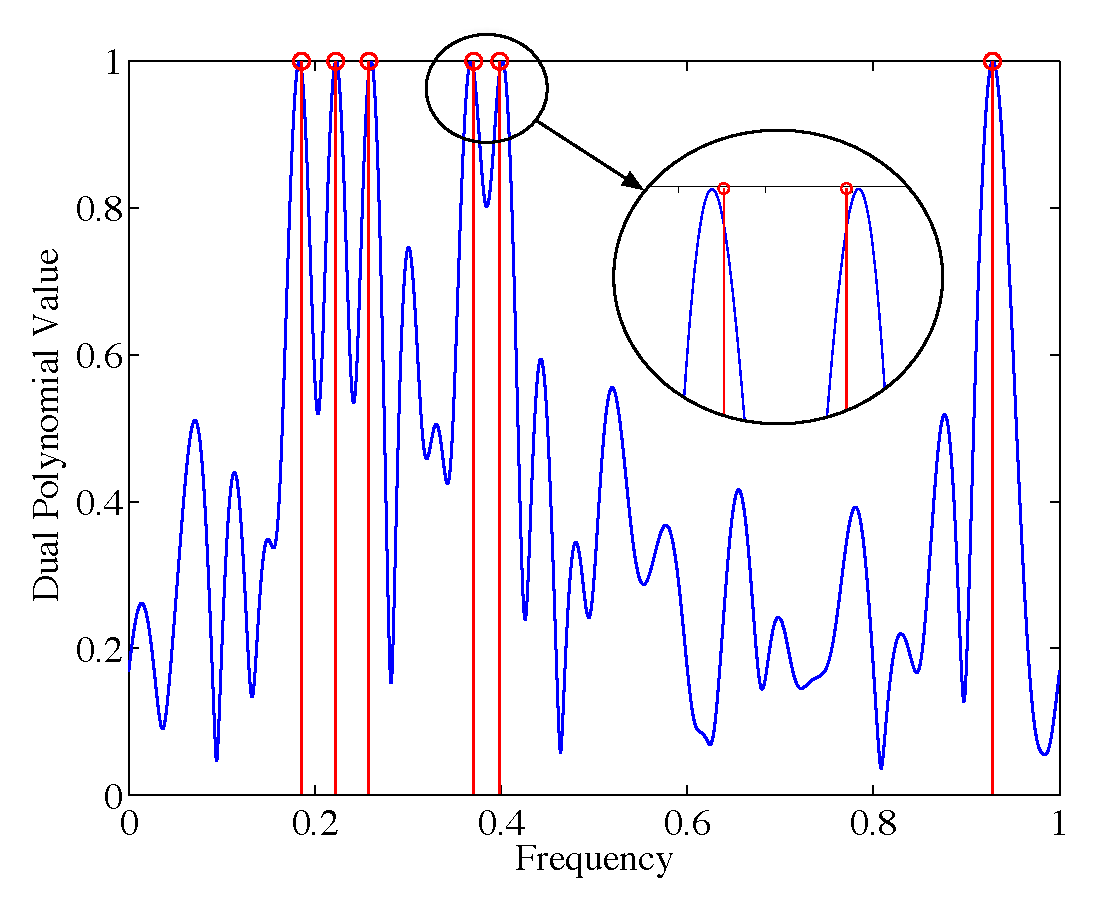
\includegraphics[width=4in]{figures/dual_poly_inset.pdf}
% \includegraphics[width=2.3in]{figures/dual_poly_inset2}
\caption{ \textbf{Frequency Localization using Dual Polynomial}: The
actual location of the frequencies in the line spectral signal $x^\star \in
\C^{64}$ is shown in red. The blue curve is the dual polynomial
obtained by solving \eqref{eq:dual-ast} with $y = x^\star + w$ where $w$ is noise of SNR 10 dB.}

\label{fig:dual_poly_localize}
\end{figure}

As shown in Corollary~\ref{cor:dual-cert-support}, the dual solution can be
used to identify the frequencies of the primal solution. For line spectra, a frequency
$f \in [0,1]$ is in the support of the solution $\hat{x}$ of \eqref{eq:linespect:ast} if and
only if
\[
	 |\langle \hat{z}, a_{f,\phi} \rangle| =\left|\ \sum_{l=0}^{n-1} \hat{z}_l e^{-i 2\pi l f} \right| = \tau
\]
That is, $f$ is in the support of $\hat{x}$ if and only if it is a point of maximum modulus for the dual polynomial. Thus, the support
may be determined by finding frequencies $f$ where the dual polynomial attains magnitude $\tau$. 

Figure~\ref{fig:dual_poly_localize} shows the dual
polynomial for $\eqref{eq:linespect:ast}$ with $n = 64$ samples and $k = 6$
 randomly chosen frequencies. The regularization
parameter $\tau$ is chosen as described in Section \ref{subsec:parameter}.

\section{Choosing the regularization parameter}\label{subsec:parameter}
The choice of the regularization parameter is dictated by the noise model and
we show the optimal choice for white gaussian noise samples in our analysis. As
noted in Theorem~\ref{cor:expected-mse}, the optimal choice of the
regularization parameter depends on the dual norm of the noise.  A simple
lower bound on the expected dual norm occurs when we consider the maximum
value of $n$ uniformly spaced points in the unit circle. Using the result of
\cite{lr76}, the lower bound whenever $n \geq 5$ is
\[
\sigma\sqrt{n\log(n) - \tfrac{n}{2} \log(4\pi\log(n))}\,.
\]

Using standard results on the extreme value statistics of Gaussian distribution,
we can also obtain a non-asymptotic upper bound on the expected dual norm of
noise for $n > 3$:
\[\sigma\left(1  + \frac{1}{\log(n)}\right)\sqrt{\log(n) + \log(16 \pi^3/2 \log(n))}\nonumber
\]

We show these computations in detail in the following section.

\section{Estimation of Gaussian Width}
\label{proof:dual-norm-bounds}

This section derives non-asymptotic upper and lower bounds on the expected dual norm of gaussian noise vectors, which are asymptotically tight upto $\log\log$ factors. Recall that the dual atomic norm of $w$ is given by $\sqrt{n}\sup_{f \in [0,1]}|W_f|$ where
\begin{equation*}
\label{ranproc}
W_f = \frac{1}{\sqrt{n}}\sum_{m=0}^{n-1}{w_m e^{-i2 \pi m f}}.
\end{equation*}

Here, the noise variables $w_1, w_2, \ldots$ are circularly symmetric
independent sequence of standard complex normal variables.

If we define two independent $i.i.d$ sequences of standard normal numbers $\{
g_k\}_1^\infty$ and $\{h_k\}_1^\infty$, note that we can write
\begin{equation}
W_f = \frac{1}{\sqrt{2 n}} \sum_{k=0}^{n-1} \left[ g_k \cos(2 \pi k f) - h_k \sin(2\pi k f) \right].
\end{equation}
Note that $W_f$ is a normal random variable with zero mean and a variance of
$1/2$.

\subsection{Upper Bound}

Let us use a $1/N$-net of the torus $\mathbb{T}$ to estimate the expectation of
$\sup_{f \in \mathbb{T}} {W_f}$. Define

\begin{equation*}
\mathbb{T}_ = \left\{t \in \mathbb{T} ~ \middle| ~ \abs{t-k/N} \leq 1/N \right\}.
\end{equation*}

We have
\begin{align}
\nonumber\E\left[\sup_{f \in T} W_f \right] & \leq \E\left[\sup_{1 \leq k \leq N} W_{k/N} \right] + \E\left[\sup_{f \in \mathbb{T}_k} \left(W_{f} - W_{k/N}\right) \right]\\
& \leq \sqrt{\log(N)} + \frac{2 \pi n}{\sqrt{3}N} \E\left[\sup_{f \in \mathbb{T}_k} Y_f \right]\label{balance}
\end{align}
where 
\begin{equation}
Y_f = \frac{\sqrt{3} N  \left(W_f - W_{k/N}\right)}{4 \pi n}.
\end{equation}
We will now use Dudley's integral inequality to bound $\E\left[\sup_{f \in \mathbb{T}_k} Y_f \right]$. To proceed, note that the distance between indices $t$ and $s$ in $\mathbb{T}_k$ is given by
\begin{align*}
\rho^2(t,s) & := \E \abs{Y_t - Y_s}^2\\
& = \frac{3 N^2}{8 \pi^2 n^2} \E \abs{X_t - X_s}^2\\
& = \frac{3 N^2}{2 \pi^2 n^3} \sum_{k=0}^{n-1}{\sin^2(\pi k (t - s))}\\
& \leq N^2 (t-s)^2.
\end{align*}

Thus, the diameter of the set $\mathbb{T}_k$
\begin{align*}
\diam_\rho(\mathbb{T}_k) &:= \sup_{t,s  \in \mathbb{T}_k}\rho(t,s) = 1\\
\end{align*}
Consequently the number $N(\mathbb{T}_k, \rho, \epsilon)$ of $\epsilon$ balls needed to cover $T_k$ under this metric $\rho$ is $1/\epsilon$. Now, by the application Dudley's integral inequality, we have
\begin{align}
\E\left[\sup_{t \in \mathbb{T}_k} Y_f \right] & \leq 24 \int_0^{\diam_\rho(T_k)} \sqrt{N(\mathbb{T}_k, \rho, \epsilon)} d\epsilon\\
 & \leq 24 \int_0^1 \sqrt{\log(1/\epsilon)} d\epsilon = 12 \sqrt{\pi}. \label{dudley}
\end{align}
Thus, from \eqref{dudley} and \eqref{balance}, we have
\begin{align*}
\E\left[\sup_{f \in \mathbb{T}} W_f \right] & \leq  \sqrt{\log(N)} +  \frac{ 16 \pi^{3/2} n} { N}
\end{align*}


Substituting $N = 16 n \sqrt{\pi^3 \log(n)},$ we get
\[
	\E\left[\sup_{f \in \mathbb{T}} W_f \right] \leq \left( 1 + \frac{1}{\log(n)} \right)\sqrt{\log(n) + \log(16 \pi^{3/2} \log(n))}
\]
\subsection{Lower Bound}

The covariance function of $W_f$ is
\begin{align*}
\E\left[W_{f_1} W_{f_2}^*\right] &= \frac{1}{n}\sum_{m=0}^{n-1} \exp(2\pi m (f_1 - f_2)) = e^{\pi (n - 1) (f_1-f_2)} \frac{\sin(n \pi (f_1 - f_2) ) }{ n \sin(\pi (f_2 - f_2))}.
\end{align*}
Thus, the $n$ samples $\left\{W_{m/n}\right\}_{m=0}^{n-1}$ are uncorrelated and thus independent because of their joint gaussianity. This gives a simple non-asymptotic lower bound using the known result for maximum value of $n$ independent gaussian random variables~\cite{lr76} whenever $n > 5$:
\begin{align*}
\E\left[\sup_{t \in T} \left| W_t \right| \right] &\geq \E\left[\max_{m = 0, \ldots, n-1} \Re\left( W_{m/n} \right)  \right] = \sqrt{\log(n) - \tfrac{ \log\log(n) + \log(4\pi)}{2}}.
\end{align*}

Combining this result with the upper bound, we have shown that the lower bound is asymptotically tight neglecting $\log\log$ terms.

% Since the dual norm induced by  $\A_N$ approximates the dual norm induced by $\A$, (See \ref{proof:dual-norm-approximation}), it is sufficient to compute an upper bound for $\vnorm{w}_{\A_N}^*.$ Note that $|W_f|^2$ has a chi-square distribution since $W_f$ is a Gaussian process. We establish a simple lemma about the maximum of chi-square distributed random variables.
% \begin{lemma}
% \label{lem:max-chi}
% Let $x_1,\ldots,x_N$ be complex gaussians with unit variance. Then,
% \begin{equation*}
% \E\left[\max_{1\leq i\leq N} |x_i|\right] \leq \sqrt{\log(N) + 1}.
% \end{equation*}
% \begin{proof}
% Let $x_1,\ldots,x_N$ be complex Gaussians with unit variance: $\E[ |x_i|^2]=1$.  Note that $2|x_i|^2$ is a chi-squared random variable with two degrees of freedom.   Using Jensen's inequality, also observe that
% \begin{align}\label{eq:jensen-bound}
% 	\E\left[\max_{1\leq i\leq N} |x_i|\right] & \leq  
% 	\E\left[\max_{1\leq i\leq N} |x_i|^2\right]^{1/2} \leq  
% 	\tfrac{1}{\sqrt{2}}\E\left[\max_{1\leq i\leq N} 2|x_i|^2\right]^{1/2}.
% \end{align}
% 
% Now let $z_1,\ldots, z_n$ be chi-squared random variables with $2$ degrees of freedom.  Then we have
% \begin{align*}
% 	\E\left[\max_{1\leq i\leq N} z_i\right] &= \int_0^\infty P\left[ \max_{1\leq i\leq N} z_i \geq t \right] dt\\
% 	\leq & \delta + \int_\delta^\infty P\left[ \max_{1\leq i\leq N} z_i \geq t \right] dt\\
% 	\leq & \delta +  N \int_\delta^\infty P\left[  z_1 \geq t\right] dt\\
% 	= & \delta +  N \int_\delta^\infty   \exp(-t/2) dt\\
% 	= & \delta +  2N  \exp(-\delta/2)
% \end{align*}
% Setting $\delta = 2\log(N)$ gives $\E\left[\max_{1\leq i\leq N} z_i\right] \leq 2 \log{N} + 2$.  Plugging this estimate into~\eqref{eq:jensen-bound} gives $\E\left[\max_{1\leq i\leq N} |x_i|\right] \leq  \sqrt{\log{N}+1}$.
% \end{proof}
% \end{lemma}
% Using Lemma \ref{lem:max-chi}, we can compute
% \begin{align*}
% \vnorm{w}_{\A_N}^* & = \sqrt{n}\max_{m=0,\ldots,N-1} \left| W_n\left(e^{i 2 \pi m/N}\right) \right|  \leq \sigma\sqrt{n\left(\log{N}+1\right)}
% \end{align*}
% Plugging in $N = 4\pi n \log(n)$ and using \eq{maximum-modulus} and
% \eq{grid-approx} establishes a tight upper bound.

\section{Universal Mean Squared Error Guarantee}

We can set the regularization parameter $\tau$ equal to an upper bound on the
expected dual atomic norm, i.e.,
\begin{equation}
\label{eq:tau}
\tau = \sigma\left(1  +  \frac{1}{\log(n)}\right)\sqrt{n \log(n) + n\log(4\pi\log(n))}.
\end{equation}
and apply Theorem \ref{cor:expected-mse} to guarantee Mean-Squared Error
consistency of AST for Line spectral Estimation. Doing so yields the asymptotic
result in Theorem \ref{thm:expmsels}. However, as noted in
Section~\ref{sec:convergence-rate}, faster convergence rates may be possible
under some conditions.

A recent result by Candes and Fernandez-Granda~\cite{CandesGranda} establishes
that in the noiseless case, the frequencies localized by the dual polynomial are
exact provided the minimum separation between the frequencies is at least $4/n$
where $n$ is the number of samples in the line spectral signal. Under similar
separation condition, numerical simulations suggest that \eqref{eq:linespect:ast} achieves
approximate frequency location in the noisy case.

In fact, we can also theoretically show that signals with well separated
frequencies are well behaved and achieve faster convergence rates. Unlike
previous work on fast rates for Lasso, our condition is on the signal instead of
the measurement operator. In fact, as frequencies can be arbitrarily close, the
measurement operator which samples line spectral signals is highly coherent and
it may be impossible to achieve robust recovery if frequencies can be close to
each other.



\section{What is the best rate we can expect?}\label{sec:minimax}

Using results about minimax achievable rates for linear models~
\cite{cd_minimax,rw_minimax}, we can deduce that the convergence rate stated in
\eqref{fast-rate} is near optimal. Define the set of $k$ well separated
frequencies as

\[
\mathcal{S}_k = \left\{(f_1, \dots, f_k) \in \mathbb{T}^k ~\middle|~  d(f_p, f_q) \geq 4/n, p \neq q \right\}
\]

The expected minimax denoising error $M_k$ for a line spectral signal with
frequencies from $\mathcal{S}_k$ is defined as the lowest expected denoising
error rate for any estimate $\hat{x}(y)$ for the worst case signal $x^\star$
with support $T(x^\star) \in \mathcal{S}_k$. Note that we can lower bound $M_k$
by restricting the set of candidate frequencies to smaller set. To that end,
suppose we restrict the signal $x^\star$ to have frequencies only drawn from an
equispaced grid on the torus $T_n := \{ 4 j/n \}_{j=1}^{n/4}$. Note that any set
of $k$ frequencies from $T_n$ are pairwise separated by at least $4/n$. If we
denote by $F_n$ a $n \times (n/4)$ partial DFT matrix with (unnormalized)
columns corresponding to frequencies from $T_n$, we can write $x^\star = F_n
c^\star$ for some $c^\star$ with $\vnorm{c^\star}_0 = k$. Thus,

\begin{align*}
M_k &:= \inf_{\hat{x}}
 \sup_{
	T(x^\star) \in \mathcal{S}_k}
\frac{1}{n} \mathbb{E} \vnorm{\hat{x} - x^\star}_2^2
	\\
&\geq \inf_{\hat{x}} 
 \sup_{
	\vnorm{c^\star}_0 \leq k
	} \frac{1}{n} \mathbb{E} \vnorm{\hat{x} - F_n c^\star}_2^2\\
&\geq \inf_{\hat{c}}
 \sup_{\vnorm{c^\star}_0 \leq k} \frac{1}{n} \mathbb{E} \vnorm{F_n(\hat{c} - c^\star)}_2^2\\
&\geq  \frac{n}{4} \left\{ \inf_{\hat{c}}
 \sup_{\vnorm{c^\star}_0 \leq k}\frac{4}{n} \mathbb{E} \vnorm{\hat{c} - c^\star}_2^2\right\}\,.
\end{align*}

Here, the first inequality is the restriction of $T(x^\star)$. The second
inequality follows because we project out all components of $\hat{x}$ that do
not lie in the span of $F_n$. Such projections can only reduce the Euclidean
norm. The third inequality uses the fact that the minimum singular value of
$F_n$ is $n$ since $F_n^*F_n = n I_{{n}/{4}}$. Now we may directly apply the
lower bound for estimation error for linear models derived by Cand\'es and
Davenport. Namely, Theorem 1 of~\cite{cd_minimax} states that

\begin{align*}
\inf_{\hat{c}}
 \sup_{\vnorm{c^\star}_0 \leq k} \frac{4}{n} \mathbb{E} \vnorm{\hat{c} - c^\star}_2^2&\geq {C} \sigma^2 \frac{k \log\left(\frac{n}{4k}\right)}{\vnorm{F_n}_\mathrm{F}^2}\,.
 \end{align*} With the preceding analysis and the fact that $\vnorm{F_n}_{\mathrm{F}}^2 = n^2/4$, we can thus deduce the following theorem:
 \begin{theorem}
\label{minimax}
Let $x^\star$ be a line spectral signal as described by \eqref{eq:signal} with the support $T(x^\star) = \{f_1, \dots, f_k\} \in \mathcal{S}_k$ and $y = x^\star + w$, where $w \in \C^n$ is circularly symmetric Gaussian noise with variance $\sigma^2 I_n$. Let $\hat{x}$ be any estimate of $x^\star$ using $y$. Then,
\[
M_k = \inf_{\hat{x}}
 \sup_{
	T(x^\star) \in \mathcal{S}_k}
\frac{1}{n} \mathbb{E} \vnorm{\hat{x} - x^\star}_2^2
\geq C\sigma^2 \frac{k \log\left(\frac{n}{4k}\right)}{n}
\]
for some constant $C$ that is independent of $k$, $n$, and $\sigma$.
\end{theorem}

This theorem and Theorem~\ref{main} certify that AST is nearly minimax optimal for spectral estimation of well separated frequencies. 

\section{Proofs for well separated frequencies}
\label{sec:proofs}

In this section, there are many numerical constants. Unless otherwise specified,
$C$ will denote a numerical constant whose value may change from equation to
equation. Specific constants will be highlighted by accents or subscripts.

We describe the preliminaries and notations, and restate some recent results we
used before sketching the proof of Theorems \ref{main} and \ref{support}.

\subsection{Preliminaries}
The sample $x^\star_j$ may be regarded as the $j$th trigonometric moment of 
the discrete measure $\mu$ given by \eqref{mu}:
\begin{eqnarray*}
  x_j^\star & = & \int_0^1 e^{i 2 \pi j f} \mu ( d f)
\end{eqnarray*}
for $-m \leq j \leq m$.
Thus, the problem of extracting the frequencies and amplitudes from noisy 
observations may be regarded as the inverse problem of estimating a measure 
from noisy trigonometric moments.

We can write the vector $x^\star$ of observations $[x_{-m}^\star, \ldots, x_m^\star]^T$ in terms of an \emph{atomic decomposition}
\[
x^\star = \sum_{l=1}^k c_l a(f_l)
\]
or equivalently in terms of a corresponding \emph{representing measure} $\mu$ given by \eqref{mu} satisfying
\[
x^\star = \int_0^1 a(f) \mu(df)
\]
There is a one-one correspondence between atomic decompositions and representing measures. Note that there are infinite atomic decompositions of $x^\star$ and also infinite corresponding representing measures. However, since every collection of $n$ atoms is linearly independent, $\A$ forms a full spark frame~\cite{spark} and therefore the problem of finding the sparsest decomposition of $x^\star$ is well-posed if there is a decomposition which is at least $n/2$ sparse.

The atomic norm of a vector $z$ defined in \eqref{def-atnorm} is the minimum total variation norm~\cite{cs_otg,tvnorm} $\vnorm{\mu}_{\mathrm{TV}}$ of all representing measures $\mu$ of $z$. So, minimizing the total variation norm is the same as finding a decomposition that achieves the atomic norm.

\subsection{Dual Certificate and Exact Recovery}

Atomic norm minimization attempts to recover the sparsest decomposition by
finding a decomposition that achieves the atomic norm, i.e., find ${c_l,f_l}$
such that $x^\star = \sum_l c_l a(f_l)$ and $ \vnorm{x^\star}_\A = \sum_l |c_l|
$ or equivalently, finding a representing measure $\mu$ of the form \eqref{mu}
that minimizes the total variation norm $ \vnorm{\mu}_{\mathrm{TV}}$. The
authors of~\cite{cg_exact12} showed that when $n > 256$, the decomposition that
achieves the atomic norm is the sparsest decomposition by explicitly
constructing a dual certificate~\cite{dualcert} of optimality, whenever the
composing frequencies $f_1, \ldots, f_k$ satisfy a minimum separation
condition~\eqref{min-sep}. In the rest of the chapter, we always make the
technical assumption that $n > 256$.

\begin{definition}[Dual Certificate]
\label{dual-cert}
A vector $q \in \C^n$ is called a dual certificate for $x^\star$ if for the corresponding trigonometric polynomial $Q(f) := \langle q, a(f) \rangle$, we have
$$Q(f_l) = \operatorname{sign}(c_l), l = 1, \ldots, k$$  and $$|Q(f)| < 1$$ whenever $f\not\in \{ f_1, \ldots, f_k\}$.
\end{definition}
The authors of ~\cite{cg_exact12} not only explicitly constructed 
such a certificate characterized by the dual polynomial $Q$, but also showed that their construction satisfies some stability conditions, which is crucial for showing that denoising using the atomic norm provides stable recovery in the presence of noise.

\begin{theorem}[Dual Polynomial Stability, Lemma 2.4 and 2.5 in \cite{cg_noisy}]
\label{dual-stab} For any $f_1, \ldots, f_k$ satisfying the separation condition \eqref{min-sep} and any sign vector $v \in \C^k$ with $|v_j|=1$, there exists a trigonometric polynomial $Q = \left<q, a(f)\right>$ for some $q \in \C^n$ with the following properties: 
\begin{enumerate}
\item For each $j = 1, \ldots, k$, $Q$ interpolates the sign vector $v$ so that $Q(f_j) = v_j$
\item In each neighborhood $N_j$ corresponding to $f_j$ defined by
$N_j = \left\{ f : d(f, f_j) < {0.16}/{n} \right\}$, 
the polynomial $Q(f)$ behaves like a quadratic and there exist constants $C_a, C_a'$ so that
\begin{align}
\label{q1}|Q(f)| & \leq 1 - \frac{C_a}{2} n^2 (f-f_j)^2\\
\label{q2}|Q(f) - v_j| & \leq \frac{C_a'}{2} n^2 (f - f_j)^2
\end{align}
\item When $f \in F = [0,1] \backslash \cup_{j=1}^k{N_j}$, there is a numerical constant $C_b>0$ such that
\[
|Q(f)| \leq 1 - C_b
\]
\end{enumerate}
\end{theorem}

We use results in~\cite{cg_noisy} and~\cite{btr12} (reproduced in Appendix D for
convenience) and borrow several ideas from the proofs in~\cite{cg_noisy}, with
nontrivial modifications to establish the error rate of atomic norm
regularization.

\subsection{Near optimal MSE}

In this section, we will prove Theorem~\ref{main}. Let $\hat{\mu}$ be the
representing measure for the solution $\hat{x}$ of \eqref{AST} with
minimum total variation norm, that is,
\[
\hat{x} = \int_0^1 a(f) \hat{\mu}(df)
\]

and $\vnorm{\hat{x}}_\A = \vnorm{\hat{\mu}}_{\mathrm{TV}}$. Denote the error
vector by $e = x^\star - \hat{x}$. Then, the difference measure $\nu = \mu -
\hat{\mu}$ is a representing measure for $e$. We first express the denoising
error $\vnorm{e}_2^2$ as the integral of the error function $E(f) = \langle e,
a(f) \rangle,$ against the difference measure $\nu$:

\begin{align*}
\vnorm{e}_2^2 &= \langle e, e \rangle\\
& = \left\langle e, \int_0^1 a(f) \nu(df) \right\rangle\\
& =  \int_0^1  \left\langle e,a(f) \right\rangle \nu(df)\\
& = \int_0^1 E(f) \nu(df).
\end{align*}


Using a Taylor series approximation in each of 
the near regions $N_j$, we first show that the denoising error (or in general any 
integral of a trigonometric polynomial against the difference measure) can be controlled in terms 
of an integral in the far region $F$ and the zeroth, first, and second 
moments of the difference measure in the near regions.  The precise result is presented in the following lemma, whose proof is given in Appendix \ref{apx:pf:taylor}.
\begin{lemma}
\label{part1}
Define
\begin{align*} 
I_0^j &:= \left| \int_{N_j} \nu(df) \right|\\
I_1^j &:= n \left| \int_{N_j} (f-f_j) \nu(df) \right|\\
I_2^j &:= \frac{n^2}{2} \int_{N_j} (f-f_j)^2 |\nu|(df)\\
I_l &:= \sum_{j=1}^k I_l^j,~~\mbox{for}~l = 0, 1, 2\,.
\end{align*}
Then for any $m$th order trigonometric polynomial $X$, we have
\[
\int_0^1{ X(f) \nu(df)}
\leq \vnorm{X(f)}_\infty \left(\int_F{|\nu|(df)} + I_0 + I_1 + I_2\right)
\]
\end{lemma}
\begin{proof}\label{apx:pf:taylor}
We first split the domain of integration into the near and far regions.
\begin{align}
\left |\int_0^1 X(f) \nu(df)\right | 
&\leq \left |\int_F X(f) \nu (f)\right | + \sum_{j=1}^k \left | \int_{N_j}X(f) \nu(df)\right |\nonumber \\
&\leq \vnorm{X(f)}_\infty \int_F |\nu| (df) + \sum_{j=1}^k \left | \int_{N_j}X(f) \nu(df) \right |.\label{Xfbd}
\end{align}
by using H\"{o}lder's inequality for the last inequality. Using Taylor's theorem, we may expand the integrand $X(f)$ around $f_j$ as
\[
X(f) = X(f_j) + (f-f_j) X'(f_j) + \frac{1}{2} X''(\xi_j) (f-f_j)^2 
\]
for some $\xi_j \in N_j$. 
Thus,
{\small
\begin{align*}
&|X(f)-X(f_j)-X'(f_j)(f-f_j)|\\
&\leq \sup_{\xi \in N_j} \frac{1}{2}|X''(\xi)|(f -f_j)^2\\ &\leq \frac{1}{2} n^2 \vnorm{X(f)}_\infty(f - f_j)^2, 
\end{align*}
}
where for the last inequality we have used a theorem of Bernstein for trigonometric polynomials (see, for example~\cite{bernstein}):  
\begin{align*}
|X'(f_j)|  & \leq n \vnorm{X(f)}_\infty\\
|X''(f_j)| & \leq n^2 \vnorm{X(f)}_\infty.
\end{align*}
As a consequence, we have
\begin{align*}
\left | \int_{N_j} X(f) \nu(df)\right| &\leq \left| X(f_j)\right| \left| \int_{N_j} \nu (df)\right| + \left|X'(f_j)\right| \left|\int_{N_j} (f-f_j) \nu (df)  \right|\\
& + \frac{1}{2} n^2 \|X(f)\|_\infty \int_{N_j} (f-f_j)^2 |\nu| (df) \\
& \leq \|X(f)\|_\infty \left(I_0^j + I_1^j + I_2^j\right).
\end{align*}
Substituting back into \eqref{Xfbd} yields the desired result.
\end{proof}


Applying Lemma \ref{part1} to the error function, we get
\begin{equation}
\label{ebd}
\vnorm{e}_2^2 \leq \vnorm{E(f)}_\infty 
\left( \int_F{|\nu|(df)} + I_0 + I_1 + I_2\right)
\end{equation}
As a consequence of our choice of $\tau$ in \eq{tau}, we can show that $\vnorm{E(f)}_\infty \leq (1+2\eta^{-1})\tau$ with high probability. In fact, we have
\begin{align*}
\vnorm{E(f)}_\infty &= \sup_{f \in [0,1]}\left|\langle e, a(f) \rangle\right|\\
&= \sup_{f \in [0,1]} \left| \langle x^\star - \hat{x}, a(f) \rangle\right|\\
&\leq \sup_{f \in [0,1]} \left| \langle w, a(f) \rangle \right| +  \sup_{f \in [0,1]} \left| \langle y - \hat{x}, a(f) \rangle \right|\\
&\leq \sup_{f \in [0,1]} \left| \langle w, a(f) \rangle \right| +  \tau\\
\label{errbd} \numberthis &\leq (1 +2\eta^{-1})\tau \leq 3 \tau, \text{with high probability.}
\end{align*}
The second inequality follows from the optimality conditions for \eqref{AST}. It is shown in Appendix C of ~\cite{btr12} that the penultimate inequality holds with high probability.

Therefore, to complete the proof, it suffices to show that the other terms on the right hand side of \eqref{ebd} are $O(\frac{k\tau}{n})$.  While there is no exact frequency recovery in the presence of noise, we can hope to get the frequencies approximately right. Hence, we expect that the integral in the far region can be well controlled and the local integrals of the difference measure in the near regions are also small due to cancellations. Next, we utilize the properties of the dual polynomial in Theorems~\ref{dual-stab} and another polynomial given in Theorem~\ref{dual-lin}  in Appendix \ref{apx:collection} to show that the zeroth and first moments of $\nu$ may be controlled in terms of the other two quantities in \eqref{ebd} to upper bound the error rate. The following lemma is similar to Lemmas 2.2 and 2.3 in~\cite{cg_noisy}, but we have made several modifications to adapt it to our signal and noise model. For completeness, we provide the proof in Appendix \ref{apx:pf:I0I1}. 

\begin{lemma}
\label{part2}
There exists numeric constants $C_0$ and $C_1$ such that
\begin{align*}
I_0 &\leq C_0 \left(\frac{k \tau}{n} + I_2 + \int_F{|\nu|(df)}\right) \\
I_1 &\leq C_1 \left(\frac{k \tau}{n} + I_2 + \int_F{|\nu|(df)}\right).
\end{align*}
\end{lemma}
\begin{proof}
\label{apx:pf:I0I1}
Consider the polar form
\[
  \int_{N_j} \nu ( df)  =  \left| \int_{N_j} \nu ( df) \right| e^{i \theta_j} .
\]
Set $v_j = e^{-i \theta_j}$ and let $Q(f)$ be the dual polynomial promised by Theorem \ref{dual-stab} for this $v$. Then, we have 
\begin{align*}
  \left| \int_{N_j} \nu ( d f) \right| & = 
  \int_{N_j} e^{- i \theta_j} \nu ( d f)\\
  & =  \int_{N_j} Q ( f) \nu ( d f) + 
  \int_{N_j} (e^{- i \theta_j} -  Q ( f) ) \nu ( d f)
\end{align*}
Summing over $j=1,\ldots,k$ yields

\begin{align}
\nonumber I_0 &= \sum_{j=1}^k \left| \int_{N_j} \nu(df) \right|\\
\nonumber & = \sum_{j=1}^k\int_{N_j} Q ( f) \nu ( d f) + 
\sum_{j=1}^k \int_{N_j} ( v_j - Q ( f)) \nu ( d f)\\
\nonumber & \leq \left|\int_0^1 Q(f) \nu(df) \right| + \int_F|\nu|(df) + C_a' I_2, \text{ using triangle inequality and \eqref{q2}}\\
\label{i0} & \leq \frac{C k \tau}{n} + \int_F|\nu|(df) + C_a' I_2, \text{ using \eqref{qv}}.
\end{align}
We use a similar argument for bounding $I_1$ but this time use the dual polynomial $Q_1(f)$ guaranteed by Theorem \ref{dual-lin}. Again, start with the polar form
\[
  \int_{N_j} (f - f_j) \nu ( d f)  =  \left|
  \int_{N_j} (f - f_j) \nu ( d f) \right| e^{i \theta_j} = I_1^j e^{i\theta_j}/n
\]
Set $v_j = e^{-i \theta_j}$ in Theorem \ref{dual-lin} to obtain
{
\begin{align*}
  I_1^j & = 
  n\int_{N_j} e^{- i \theta_j} ( f - f_j) \nu ( d f)\\
  & =  n \int_{N_j} (v_j (
  f - f_j) - Q_1 ( f)) \nu ( d f)  + n\int_{N_j} Q_1 ( f) \nu ( d f)
\end{align*}
}
Summing over $j=1,\ldots,k$ yields
{
\begin{align}
\nonumber I_1 &= \sum_{j=1}^k I_1^j\\
\nonumber &= n \sum_{j=1}^k \int_{N_j} (v_j (
  f - f_j) - Q_1 ( f)) \nu ( d f) + n\sum_{j=1}^k\int_{N_j} Q_1 ( f) \nu ( d f)\\
\nonumber &\leq C_a^1 I_2 + n\left|\int_0^1 Q_1(f) \nu(df)\right| +  n\left |\int_F Q_1(f) \nu(df)\right |\\
\label{i1}& \leq C_a^1 I_2 + \frac{C k \tau}{n} +  C_b^1 \int_F|\nu|(df)
\end{align}
}
For the first inequality, we have used \eqref{ca1} and triangle inequality, and for the last inequality, we have used \eqref{q1v} and \eqref{cb1}. Equations \eqref{i0} and \eqref{i1} complete the proof.
\end{proof}	

All that remains to complete the proof is an upper bound on $I_2$ and $\int_F{|\nu|(df)}$.  The key idea in establishing such a bound is deriving upper and lower bounds on the
difference $\| P_{T^c} ( \nu) \|_{{\mathrm{TV}}} - \| P_T ( \nu) \|_{{\mathrm{TV}}}$
between the total variation norms of $\nu$ on and off the support. The upper bound can be derived using optimality conditions. We lower bound $\| P_{T^c} ( \nu)
\|_{{\mathrm{TV}}} - \| P_{T} ( \nu) \|_{{\mathrm{TV}}}$ using the fact that a constructed dual
certificate $Q$ has unit magnitude for every element in the support
$T$ of $P_T ( \nu)$ whence we have $\| P_T ( \nu) \|_{{\mathrm{TV}}} = \int_{\mathbb{T}}
Q ( f) \nu ( d f)$. A critical element in deriving both the lower and upper bounds is that the dual polynomial $Q$ has quadratic drop in each near regions $N_j$ and is bounded away from one in the far region $F$. Finally, by combing these bounds and carefully controlling the regularization parameter, we get the desired result summarized in the following lemma. The details of the proof are fairly technical and we leave them to Appendix \ref{apx:pf:I2far}.

\begin{lemma}
Let $\tau = \eta\sigma \sqrt{n\log(n)}$. If $\eta>1$ is large enough, then there exists a numerical constant $C$ such that, with high probability
\label{part3}
\[
\int_F{|\nu|(df)} + I_2 \leq \frac{C k \tau}{n}.
\]
\end{lemma}
\begin{proof}\label{apx:pf:I2far}
Denote by $P_T(\nu)$ the projection of the difference measure $\nu$ on the support set $T = \{f_1, \ldots, f_k\}$ of $x^\star$ so that $P_T(\nu)$ is supported on $T$. Then, setting $Q(f)$ the polynomial in Theorem \ref{dual-stab} that interpolates the sign of $P_T( \nu)$, we have
{
\begin{align*}
  \| P_T ( \nu) \|_{\mathrm{TV}} & =  \int_0^1 Q ( f) P_T ( \nu) ( d f)\\
  & \leq  \left| \int_0^1 Q ( f) \nu ( d f) \right| + \left|
  \int_{T^c} Q ( f) \nu ( d f) \right|\\
  & \leq  \frac{C k \tau}{n} + \sum_{f_j \in T} \left|
  \int_{N_j / \{ f_j \}} Q ( f) \nu ( d f) \right| + \left|
  \int_F Q ( f) \nu ( d f) \right|,
\end{align*}}
where for the first inequality we used triangle inequality and for the last inequality we used \eqref{qv}. 
The integration over $F$ is can be bounded using H\"{o}lder's inequality
\[
  \left| \int_{F} Q ( f) \nu ( d f) \right|  
  \leq  ( 1 - C_b) \int_F |\nu|(df)
\]

We continue with
{
\begin{align*}
  \left| \int_{N_j / \{ f_j \}} Q ( f) \nu ( d f) \right| 
  & \leq  \left| \int_{N_j / \{ f_j \}} | Q ( f) | | \nu | ( d f) \right|\\
  & \leq  \int_{N_j / \{ f_j \}} ( 1 - \tfrac{1}{2}n^2 C_a ( f - f_j)^2) | \nu | ( d f)\\
  & \leq \int_{N_j / \{ f_j \}} | \nu | ( d f) - C_a I_2^j.
\end{align*}
}
As a consequence, we have
{
\begin{align*}
  \nonumber \| P_T ( \nu) \|_{\mathrm{TV}} & \leq  \frac{C k \tau}{n} + \sum_{f_j
  \in T} \int_{N_j / \{ f_j \}} | \nu | ( d f) - C_a
  I_2 + ( 1 - C_b) \int_F |\nu|(df) \nonumber\\
 & \leq  \frac{C k \tau}{n} + \underbrace{\sum_{f_j
  \in T} \int_{N_j / \{ f_j \}} | \nu | ( d f) + \int_F |\nu|(df)}_{\|P_{T^c}\|_{\mathrm{TV}}} - C_a
 I_2  - C_b \int_F |\nu|(df)
\end{align*}
}
or equivalently,
\begin{align}
  \label{eqn:lower}
\|P_{T^c}(\nu) \|_{\mathrm{TV}} - \|P_T(\nu)\|_{\mathrm{TV}} \geq C_a I_2 + C_b \int_F |\nu|(df) - \frac{C k\tau}{n}.
\end{align}

Now, we appeal to Proposition \ref{pro:optimality} and obtain
\[
\vnorm{\hat{x}}_\A \leq \vnorm{x^\star}_\A - \langle w, e \rangle/\tau
\]
and thus
\begin{equation}
\label{opt-cond}
\vnorm{\hat{\mu}}_{\mathrm{TV}} \leq \vnorm{\mu}_{\mathrm{TV}} + |\langle w, e \rangle|/\tau.
\end{equation}
Using Lemma~\ref{part1},
\begin{align}
\nonumber |\langle w, e \rangle| & = |\langle w, \int_0^1 a(f) \nu(df)  |\rangle\\
& = \left|\int_0^1  \left\langle w,  a(f)  \right\rangle \nu(df)\right|\\
\nonumber & \leq \vnorm{\left\langle w,  a(f)  \right\rangle}_\infty\left(\frac{C k \tau}{n} + I_0 + I_1 + I_2\right)\\
\label{w-expand}& \leq 2\eta^{-1} \tau \left(\frac{C k \tau}{n} + I_0 + I_1 + I_2\right)\nonumber \\
 & \leq C \eta^{-1} \tau \left(\frac{k\tau}{n} + I_2 + \int_F |\nu|(df) \right)
\end{align}
with high probability, where for the penultimate inequality we used our choice of $\tau$ and $\vnorm{\left\langle w,  a(f)  \right\rangle}_\infty \leq 2\eta^{-1} \tau$ with high probability, a fact shown in Appendix C of ~\cite{btr12}. 
Substituting \eqref{w-expand} in \eqref{opt-cond}, we get
\begin{align*}
& \vnorm{\mu}_{\mathrm{TV}} + C \eta^{-1} \tau \left(\frac{k\tau}{n} + I_2 + \int_F |\nu|(df) \right)\\
& \geq \vnorm{\hat{\mu}}_{\mathrm{TV}}\\
& = \vnorm{\mu + \nu}_{\mathrm{TV}}\\
& \geq \vnorm{\mu}_{\mathrm{TV}} - \vnorm{{P_T(\nu)}}_{\mathrm{TV}} + \vnorm{{P_{T^c}(\nu)}}_{\mathrm{TV}}\end{align*}
Canceling $\|\mu\|_{\mathrm{TV}}$ yields 
\begin{align}\label{eqn:upper}
\|P_{T^c}(\nu)\|_{\mathrm{TV}} - \|P_T(\nu)\|_{\mathrm{TV}} \leq C\eta^{-1}\tau \left(\frac{k \tau}{n} + I_2 + \int_F |\nu|(df)\right)
\end{align}
As a consequence of \eqref{eqn:lower} and \eqref{eqn:upper}, we get,
\[
  C(1+\eta^{-1}) \frac{k \tau}{n} \geq  ( C_b - \eta^{-1} C)  \int_F{|\nu|(df)} + ( C_a - \eta^{-1} C)I_2
\]
whence the result follows for large enough $\eta.$
\end{proof}

Putting together Lemmas \ref{part1}, \ref{part2} and \ref{part3}, we finally prove our main theorem:
\begin{align*}
\frac{1}{n}\vnorm{e}_2^2 
&\leq \frac{\vnorm{E(f)}_\infty}{n} \left(\int_F{|\nu|(df)} + I_0 + I_1 + I_2\right)\\
&\leq \frac{\vnorm{E(f)}_\infty}{n} \left(\frac{C_1 k \tau}{n} + C_2 \int_F{|\nu|(df)} + C_3 I_2\right)\\
&\leq  \frac{\vnorm{E(f)}_\infty}{n} \frac{C k \tau}{n} \\
& \leq \frac{C k \tau^2}{n^2}\\
&= O\left(\sigma^2\frac{k \log(n)}{n}\right).
\end{align*}

The first three inequalities come from successive applications of Lemmas 1, 2
and 3 respectively. The fourth inequality follows from \eqref{errbd} and the
fifth by our choice of $\tau$ according to Eq. \eq{tau}. This completes the
proof of Theorem \ref{main}.

\subsection{Approximate Frequency Localization}
\label{sec:support}

In this section, we will prove Theorem~\ref{support}. The first two statements
in Theorem \ref{support} are direct consequences of Lemma~\ref{part3}. For
(iii.), we follow~\cite{granda2} and use the dual polynomial $Q_j^{\star} ( f) =
\langle q_j^{\star}, a ( f)\rangle$ constructed in Lemma 2.2 of~\cite{granda2}
which satisfies

\begin{eqnarray*}
  Q_j^{\star} ( f_j) & = & 1\\
  | 1 - Q_j^{\star} ( f) | & \leq & n^2 C_1' ( f - f_j)^2, f \in N_j\\
  | Q_j^{\star} ( f) | & \leq & n^2 C_1' ( f - f_{j'})^2, f \in N_{j'}, j' \neq
  j\\
  | Q_j^{\star} ( f) | & \leq & C_2', f \in F.
\end{eqnarray*}
We note that $c_j - \sum_{\hat{f}_l \in N_j} \hat{c}_l = \int_{N_j} \nu(df)$. Then, by applying triangle inequality several times,
\begin{align*}
\left| \int_{N_j}  \nu(df)\right|
& \leq \left| \int_{N_j}  Q_j^\star (f) \nu(df)\right| + \left| \int_{N_j}  (1-Q_j^\star (f)) \nu(df)\right|\\
& \leq \left| \int_0^1  Q_j^\star (f) \nu(df)\right| + \left| \int_{N_j^c}  Q_j^\star (f) \nu(df)\right| + \left| \int_{N_j}  (1-Q_j^\star (f)) \nu(df)\right|\\
& \leq \left|\int_0^1  Q_j^\star (f) \nu(df)\right| + \left| \int_{F}  Q_j^\star (f) \nu(df)\right| \\
&\qquad\qquad\qquad + \sum_{\substack{j' \neq j\\j'=1}}^k \int_{N_{j'}} \left| Q_j^\star (f)\right| |\nu|(df) +  \int_{N_j}  \left|1-Q_j^\star (f)\right| |\nu(df)|\,.
\end{align*}

We upper bound the first term using Lemma~\ref{l4} in Appendix \ref{apx:collection} which yields
\[
\left| \int^0_{1}  Q_j^\star (f) \nu(df)\right| \leq \frac{Ck \tau}{n}
\]
The other terms can be controlled using the properties of $Q_j^\star$:
\begin{align*}
\left| \int_{F}  Q_j^\star (f) \nu(df)\right| & \leq C_2' \int_{F} |\nu| (df)\\
\sum_{\substack{j' \neq j\\j'=1}}^k \int_{N_{j'}} \left| Q_j^\star (f)\right| |\nu|(df) +  \int_{N_j}  \left|1-Q_j^\star (f)\right| |\nu|(df)
& \leq
 C_1'\sum_{j'=1}^k \int_{N_{j'}} n^2 (f-f_{j'})^2 |\nu|(df) = C_1 I_2
\end{align*}
Using Lemma~\ref{part3}, both of the above are upper bounded by $\frac{C k \tau}{n}$. Now, by combining these upper bounds, we finally have
\[
\left| c_j - \sum_{l : \hat{f}_l \in N_j} \hat{c}_l \right| \leq \frac{C_3 k \tau}{n}
\]
This shows part (iii) of the theorem. Part (iv) can be obtained by combining parts (ii) and (iii).


\section{Related Work}
\label{sec:prony-method}

% \todo{Reduce Prony}
% \todo{Prony, Music, Cadzow, Matrix Pencil only 1 para}
% \todo{Discretization Malioutov and Basis Mismatch}
% \todo{Candes}

% This
% technique is attributed to Prony in the eighteenth century.

The classical methods of line spectral estimation, often called linear
prediction methods, are built upon the seminal interpolation method of
Prony~\cite{prony1795}. In the noiseless case, with as little as $n=2k$
measurements, Prony's technique can identify the frequencies exactly, no matter
how close the frequencies are. However, Prony's technique is known to be
sensitive to noise due to instability of polynomial rooting~\cite{kahn92}.
Following Prony, several methods have been employed to robustify polynomial
rooting method including the Matrix Pencil algorithm~\cite{hua02}, which
recasts the polynomial rooting as a generalized eigenvalue problem and cleverly
uses extra observations to guard against noise. The MUSIC~\cite{music} and
ESPRIT~\cite{esprit} algorithms exploit the low rank structure of the
autocorrelation matrix.


Cadzow~\cite{cadzow02} proposed a heuristic that improves over MUSIC by 
exploiting the Toeplitz structure of the matric of moments by alternately
projecting between the linear space of Toeplitz matrices and the space of rank
$k$ matrices where $k$ is the desired model order.
Cadzow's technique is very similar~\cite{ssa_special_issue} to a popular
technique in time series literature~\cite{tsbook1,tsbook2} called Singular
Spectrum Analysis~\cite{ssa}, which uses autocorrelation matrix instead
of the matrix of moments for projection. Both these techniques may be viewed as
instances of structured low rank approximation~\cite{chu2003structured} which
exploit additional structure beyond low rank structure used in subspace based
methods such as MUSIC and ESPRIT. Cadzow's method has been identified as a  fruitful preprocessing step for linear prediction methods~\cite{blu08}. A  survey of classical linear prediction methods can be found in~\cite{blu08,StoicaMoses} and an extensive list of references is given in~\cite{stoica93}.

Most, if not all of the linear prediction methods need to estimate the model
order by employing some heuristic and the performance of the algorithm is
sensitive to the model order. In contrast, our algorithms AST and the Lasso
based method, only need a rough estimate of the noise variance. In our experiments, we provide
the true model order to Matrix Pencil, MUSIC and Cadzow methods, while we use
the estimate of noise variance for AST and Lasso methods, and still compare favorably to the classical line spectral methods.

In contrast to linear prediction methods, a number of authors
~\cite{chen98spectrum,malioutov05,bourguignon2007irregular}
have suggested using compressive sensing and viewing the frequency estimation
as a sparse approximation problem. For instance,~\cite{malioutov05} notes that
the Lasso based method has better empirical localization performance than the
popular MUSIC algorithm. However, the theoretical analysis of this phenomenon
is complicated because of the need to replace the continuous frequency space by
an oversampled frequency grid. Compressive sensing based results (see, for
instance,~\cite{duartescs}) need to carefully control the incoherence of their
linear maps to apply off-the-shelf tools from compressed sensing. It is
important to note that the performance of our algorithm improves as the grid
size increases. But this seems to contradict conventional wisdom in compressed
sensing because our design matrix $\Phi$ becomes more and more coherent, and
limits how fine we can grid for the theoretical guarantees to hold.

We circumvent the problems in the conventional compresssive sensing analysis by
directly working in the continuous parameter space and hence step away from
such notions as coherence, focussing on the geometry of the atomic set as the
critical feature. By showing that the continuous approach is the limiting
case of  the Lasso based methods using the convergence of the corresponding
atomic norms, we justify denoising line spectral signals using Lasso on a
large grid. Since the original submission of this manuscript,
Cand\`es and Fernandez-Granda~\cite{CandesGranda} showed that our SDP
formulation exactly recovers the correct frequencies in the noiseless case.

To date, line spectral analysis may be broadly classified into two camps.
\emph{Subspace methods}~\cite{music,esprit,cadzow05,ssa} build upon polynomial
interpolation~\cite{prony1795} and exploit certain low rank structure in the
spectrum estimation problem for denoising. Research on subspace approaches has
yielded several standard algorithms that are widely deployed and shown to
achieve Cram\'{e}r-Rao bound asymptotically~\cite{fri,cramer-subspace}.
However, the sensitivity to noise and model order is not well understood, and
there are few guarantees of how these algorithms perform given a limited number
of noisy measurements. For a review of many of these classical approaches, see
for example~\cite{StoicaMoses}.

More recently, approaches based on convex optimization have gained favor and
have been demonstrated to perform well on a variety of spectrum estimation
tasks~\cite{malioutov05,bourguignon2007irregular,baraniuk2010model,zweig2003irregular}. These convex programming methods restrict the frequencies to lie on a
finite grid of points and view line spectral signals as a sparse combination of
single frequencies. While these methods are reported to have significantly
better localization properties than subspace methods (see for
example,~\cite{malioutov05}) and admit fast and robust algorithms, they have
two significant drawbacks. First, while finer gridding may lead to better
performance, very fine grids are often numerically unstable. Furthermore,
traditional compressed sensing theory does not adequately characterize the
performance of fine gridding in these algorithms as the dictionary becomes
highly coherent.

Some very recent work~\cite{btr12,cg_exact12,cg_noisy} bridges the gap between
the performant discretized algorithms and continuous subspace approaches by
developing a new theory of convex relaxations for infinite continuous
dictionary of frequencies. Our work in~\cite{btr12} applies the atomic norm
framework proposed by Chandrasekaran et al~\cite{crpw} to the line spectral
estimation problem. There, we established stability results on the denoising
error and demonstrated empirically that our algorithm compared favorably with
both the classical and recent convex approaches which assume the frequencies
are on an oversampled DFT grid. Our prior results made no assumption about the
separation between frequencies. When the frequencies are well separated, the
current work demonstrates that much faster convergence rates are achieved.

Our work is closely related to recent results established by Cand\`es and
Fernandez-Granda~\cite{cg_exact12} on exact recovery using convex methods and
their recent work~\cite{cg_noisy} on exploiting the robustness of their dual
polynomial construction to show super-resolution properties of convex methods.
The total variation norm formulation used in~\cite{cg_noisy} is equivalent to
the atomic norm specialized to the line spectral estimation problem.

Robustness bounds were established in both our earlier work~\cite{btr12} and in
the work of Cand\`es and Fernandez-Granda~\cite{cg_noisy}. In~\cite{btr12}, a
slow convergence rate was established with no assumptions about the separation
of frequencies in the true signal. In~\cite{cg_noisy}, the authors provide
guarantees on the $L_1$ energy of error in the frequency domain in the case
that the frequencies are well separated. The noise is assumed to be adversarial
with a small $L_1$ spectral energy. In contrast, we show near minimax
denoising error under Gaussian noise. It is also not clear that there is a
computable formulation for the optimization problem analyzed
in~\cite{cg_noisy}. While the guarantees the authors derive in~\cite{cg_noisy}
are not comparable with our results, several of their mathematical
constructions are used in our proofs here.

Additional recent work derives conditions for approximate support recovery
under the Gaussian noise model using the Beurling-Lasso ~\cite{azais}. There,
the authors show that there is a true frequency in the neighborhood of every
estimated frequency with large enough amplitude. We note that the
Beurling-Lasso is equivalent to the atomic norm algorithm that we analyze in
this chapter. A more recent paper by Fernandez-Granda{\cite{granda2}} improves
this result by giving conditions on recoverability in terms of the true signal
instead of the estimated signal and prove a theorem similar to
Theorem~\ref{support}, but use a worst case $L_2$ bound on the noise samples.
Here, we improve these recent results in our proof of Theorem~\ref{support},
providing tighter guarantees under the Gaussian noise model.
 


\section{Experiments}
\label{sec:experiments}

We compared the performance of AST, the discretized Lasso approximation, the
Matrix Pencil, MUSIC and Cadzow's method, both in terms of the mean squared
estimation error as in Theorem~\ref{main} and frequency localization. For our
experiments, we generated $k$ normalized frequencies $f_1^\star, \ldots,
f_k^\star$ uniformly randomly chosen from $\left[0,1\right]$ such that every
pair of frequencies are separated by at least $1/2n$. The signal $x^\star \in
\C^n$ is generated according to \eqref{eq:signal} with $k$ random amplitudes
independently chosen from $\chi^2(1)$ distribution (squared Gaussian). All of
our sinusoids were then assigned a random phase (equivalent to multiplying
$c_k^\star$ by a random unit norm complex number). Then, the observation $y$ is
produced by adding complex white gaussian noise $w$ such that the input signal
to noise ratio (SNR) is $-10,-5,0,5,10,15$ or $20$ dB. We compare the average
MSE of the various algorithms in 20 trials for various values of number of
observations $(n = 64,128,256)$, and number of frequencies $ (k =
n/4,n/8,n/16)$.


AST needs an estimate of the noise variance $\sigma^2$ to pick the
regularization parameter according to \eq{tau}. In many situations, this
variance is not known to us \emph{a priori}. However, we can construct a
reasonable estimate for $\sigma$ when the phases are uniformly random. It is
known that the autocorrelation matrix of a line spectral signal (see, for
example Chapter 4 in \cite{StoicaMoses}) can be written as a sum of a low rank
matrix and $\sigma^2 I$ if we assume that the phases are uniformly random. Since
the empirical autocorrelation matrix concentrates around the true expectation,
we can estimate the noise variance by averaging a few smallest eigenvalues of
the empirical autocorrelation matrix. In the following experiments, we form the
empirical autocorrelation matrix using the MATLAB routine \texttt{corrmtx} using
a prediction order $m=n/3$ and averaging the lower $25\%$ of the eigenvalues. We
used this estimate in equation~\eq{tau} to determine the regularization
parameter for both our AST and Lasso experiments.

First, we implemented AST using the ADMM method described in detail in
Chapter~\ref{chap:algos}. We used the stopping criteria described
in~\cite{admm2011} and set $\rho=2$ for all experiments. We use the dual
solution $\hat{z}$ to determine the support of the optimal solution $\hat{x}$
using the procedure described in Section~\ref{sec:frequency-localize}. Once the
frequencies $\hat{f}_l$ are extracted, we ran the least squares problem
$\mbox{minimize}_\alpha \|U \alpha - y\|^2$ where $U_{jl} = \exp(i 2\pi j
\hat{f}_l)$ to obtain a \emph{debiased} solution. After computing the optimal
solution $\alpha_{\mathrm{opt}}$, we returned the prediction $\hat{x} =
U\alpha_{\mathrm{opt}}$.

We implemented Lasso, obtaining an estimate $\hat{x}$ of $x^\star$ from $y$ by
solving the optimization problem \eqref{epsprimal} with debiasing. We use the
algorithm described in Section \ref{sec:comp-method} with grid of $N=2^{m}$
points where $m=10,11,12,13,14$ and $15$. Because of the basis mismatch effect,
the optimal $c_{\mathrm{opt}}$ has significantly more non-zero components than
the true number of frequencies. However, we observe that the frequencies
corresponding to the non-zero components of $c_{\mathrm{opt}}$ cluster
around the true ones. We therefore extract one frequency from each cluster of
non-zero values by identifying the grid point with the maximum absolute
$c_{\mathrm{opt}}$ value and zero everything else in that cluster. We then ran
a debiasing step which solves the least squares problem $\mbox{minimize}_\beta
\|\Phi_S \beta- y\|^2$ where $\Phi_S$ is the submatrix of $\Phi$ whose columns
correspond to frequencies identified from $c_{\mathrm{opt}}$. We return the
estimate $\hat{x} = \Phi_S \beta_{\mathrm{opt}}$. We used the freely
downloadable implementation of SpaRSA to solve the Lasso problem. We used a
stopping parameter of $10^{-4}$, but otherwise used the default parameters.

We implemented Cadzow's method as described by the
pseudocode in~\cite{blu08}, the Matrix Pencil as described in~\cite{hua02} and
MUSIC~\cite{music} using the MATLAB routine \texttt{rootmusic}. All these
algorithms need an estimate of the number of sinusoids. Rather
than implementing a heuristic to estimate $k$, \emph{we fed the true $k$ to our
solvers}. This provides a huge advantage to these algorithms. Neither AST or the
Lasso based algorithm are provided the true value of $k$, and the noise 
variance $\sigma^2$ required in the regularization parameter is estimated from $y$.

Let $\{\hat{c}_l\}$ and $\{\hat{f}_l\}$ denote the amplitudes and frequencies
estimated by any of the algorithms - AST, MUSIC or Cadzow. We use the following
error metrics to characterize the frequency localization of various algorithms:
\begin{enumerate} \item[(i)] Sum of the absolute value of amplitudes in the far
region $F$, $m_1 = \sum_{l : \hat{f}_l \in F} |\hat{c}_l|$ \item[(ii)] The
weighted frequency localization error, $m_2 = \sum_{l : \hat{f}_l \in N_j}
|\hat{c}_l| \{ \min_{f_j \in T} d(f_j,\hat{f}_l) \}^2$ \item[(iii)] Error in
approximation of amplitudes in the near region, $m_3 = \left| c_j - \sum_{l :
\hat{f_l} \in N_j} \hat{c}_l \right|$ \end{enumerate} These are precisely the
quantities that we prove tend to zero in Theorem~\ref{support}.

\begin{figure*}[htbp]
  \begin{tabular}{c}
	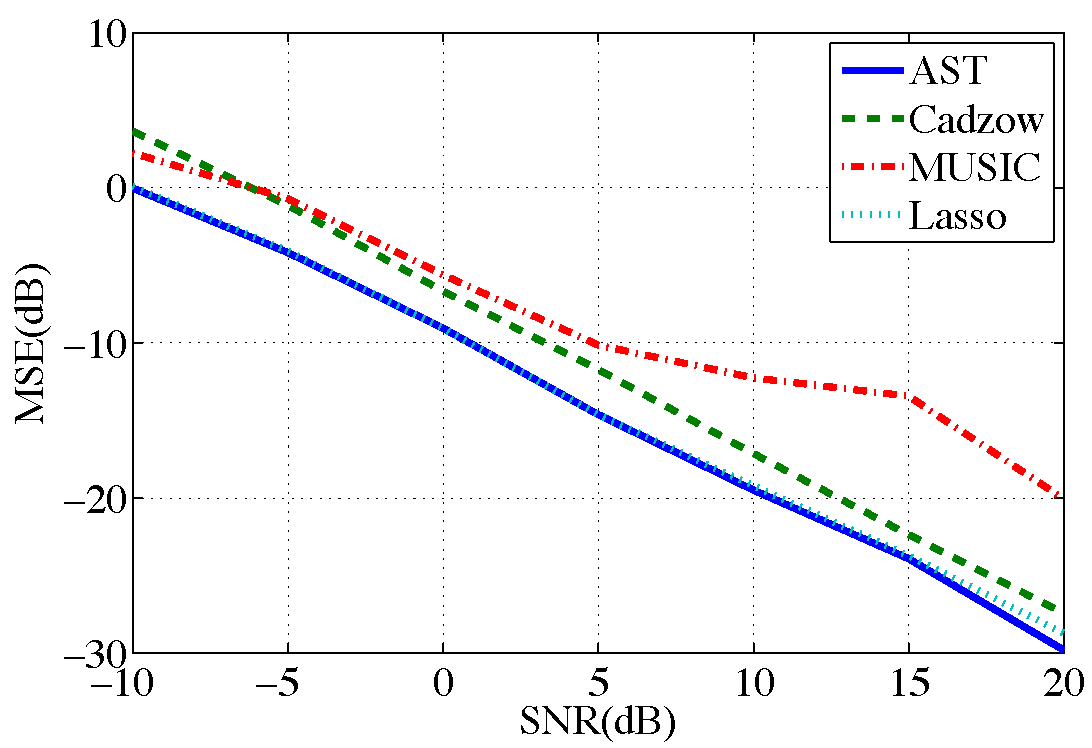
\includegraphics[width=0.5\textwidth]{figures/mse_snr_128_8_randamp}
	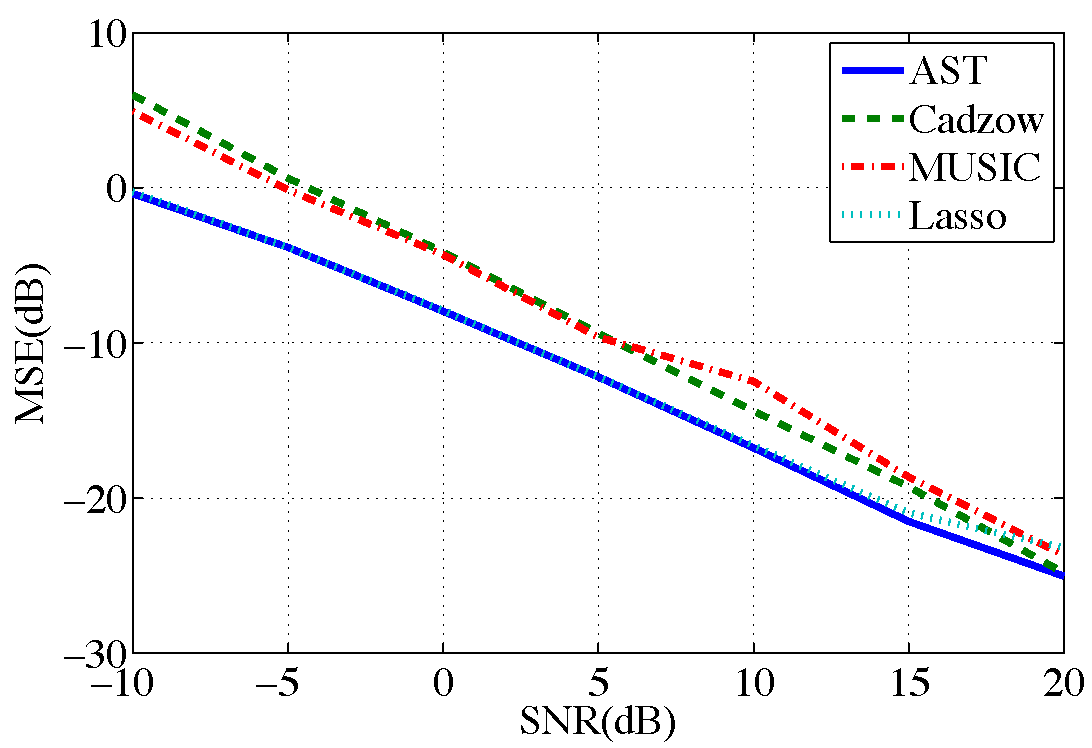
\includegraphics[width=0.5\textwidth]{figures/mse_snr_128_16_randamp} \\
	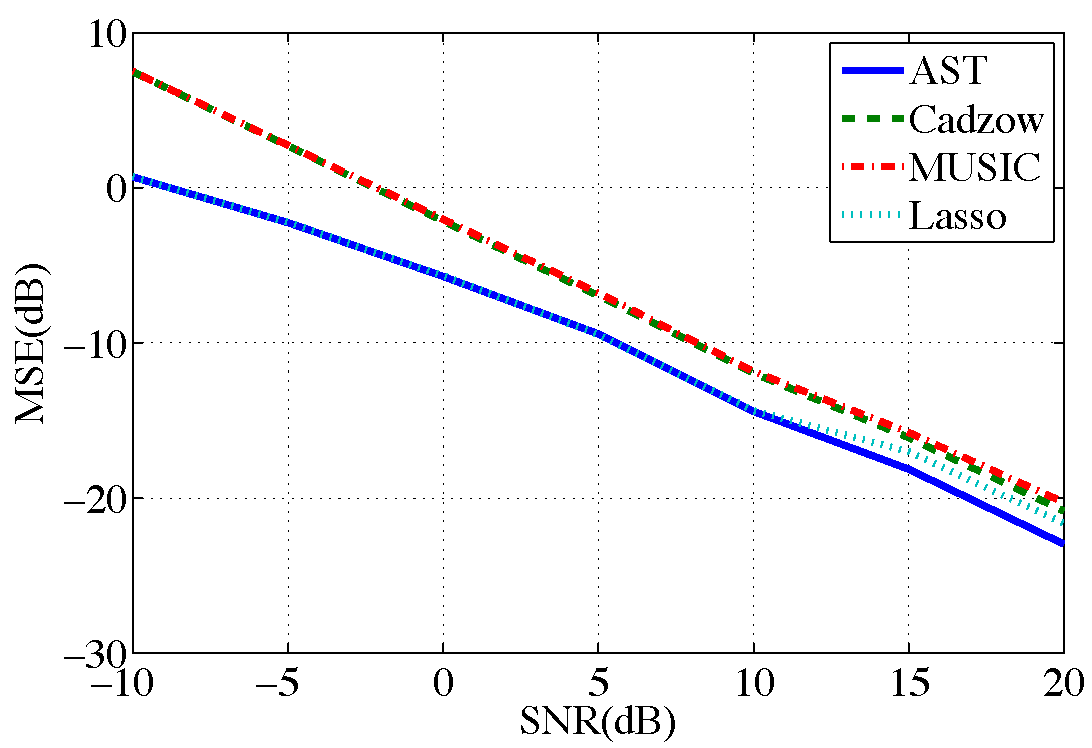
\includegraphics[width=0.5\textwidth]{figures/mse_snr_128_32_randamp}
\end{tabular}
\caption{ {\bfseries MSE vs SNR plots:} This graph compares MSE vs SNR for a subset of experiments with $n=128$ samples. From top left, clockwise, the plots are for combinations of $8$, $16$, and $32$ sinusoids with amplitudes and frequencies sampled at random.}
\label{fig:mse-snr}
\end{figure*}

In Figure~\ref{fig:mse-snr}, we show MSE vs SNR plots for a subset of
experiments when $n=128$ time samples are taken to take a closer look at the
differences. It can be seen from these plots that the performance difference
between classical algorithms such as MUSIC and Cadzow with respect to the
convex optimization based AST and Lasso is most pronounced at lower sparsity
levels. When the noise dominates the signal (SNR $\leq 0$ dB), all the
algorithms are comparable. However, AST and Lasso outperform the other
algorithms in almost every regime.


\begin{figure}[htbp]
  \begin{tabular}{cc}
	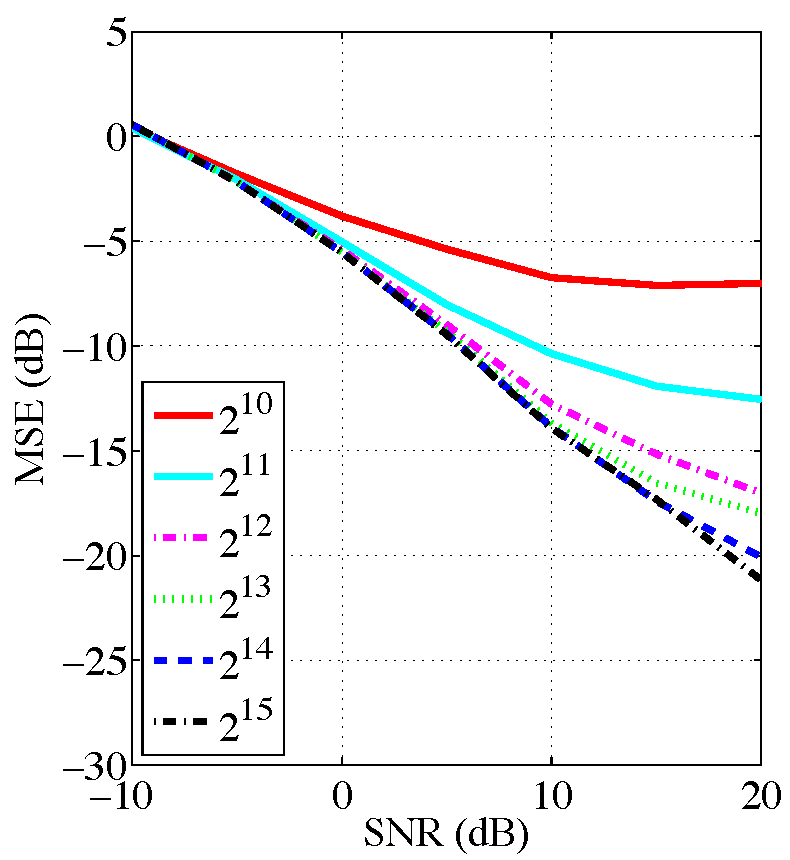
\includegraphics[trim=10mm 0mm 5mm 3mm,clip,width=0.37\linewidth]{figures/mse_snr_256_64_lasso_randamp} &
	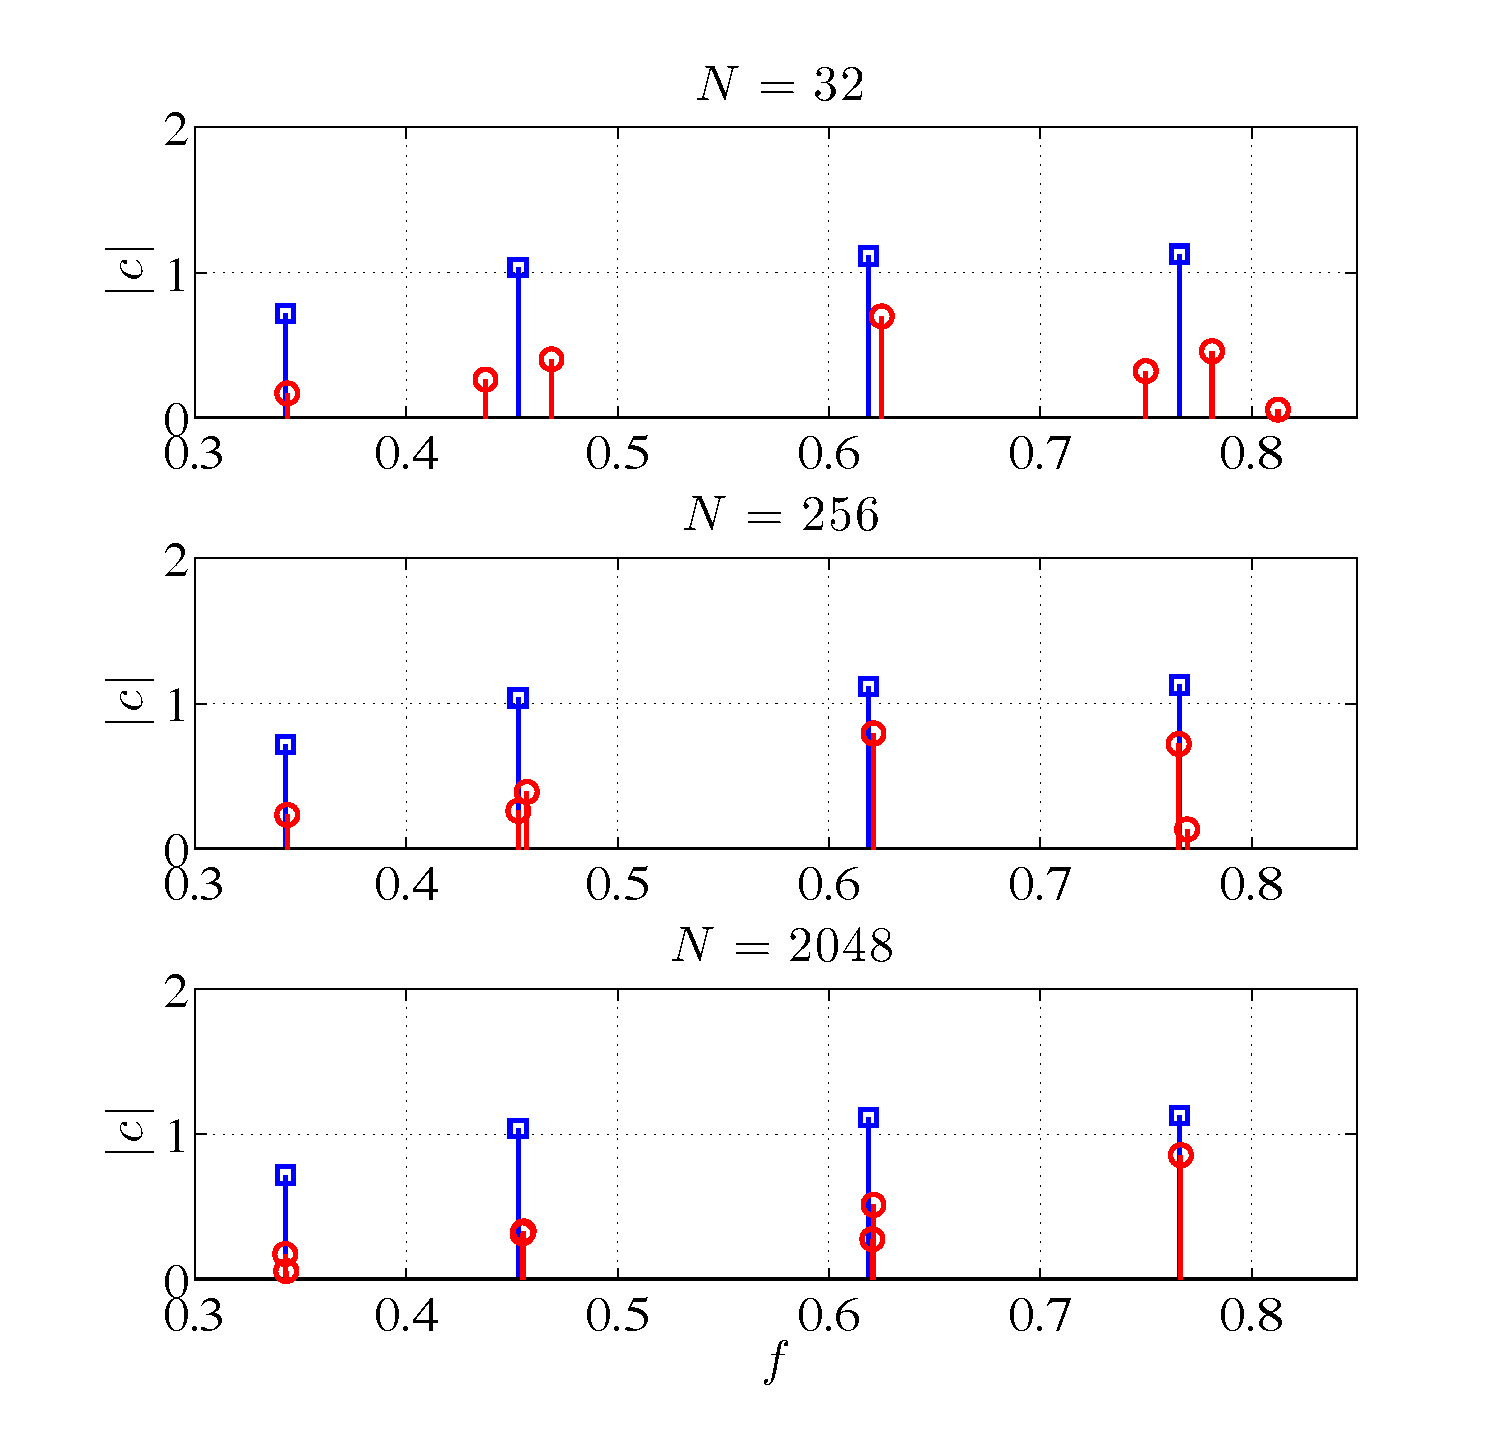
\includegraphics[trim=15mm 0mm 20mm 3mm,clip,width=0.45\linewidth]{figures/gridding} \\
(a)  & (b)
\end{tabular}
\caption{ 
(a) Plot of MSE vs SNR for Lasso at different grid sizes for a subset of experiments with $n=128, k = 16$\newline
(b) Lasso Frequency localization with $n=32, k = 4,$
SNR = $10$ dB. Blue represents the true frequencies, while red are given by Lasso. For better visualization, we threshold the Lasso solution by $10^{-6}$.}
\label{fig:lasso-compare}
\end{figure}

We note that the denoising performance of Lasso improves with increased grid
size as shown in the MSE vs SNR plot in Figure~\ref{fig:lasso-compare}(a). The
figure shows that the performance improvement for larger grid sizes is greater
at high SNRs. This is because when the noise is small, the discretization error
is more dominant and finer gridding helps to reduce this error.
Figures~\ref{fig:lasso-compare}(a) and (b) also indicate that the benefits of
increasing discretization levels are diminishing with the grid sizes, at a
higher rate in the low SNR regime, suggesting a tradeoff among grid size,
accuracy, and computational complexity.

Finally, in Figure \ref{fig:lasso-compare}(b), we provide numerical evidence
supporting the assertion that frequency localization improves with increasing
grid size. Lasso identifies more frequencies than the true ones due to basis
mismatch. However, these frequencies cluster around the true ones, and more
importantly, finer discretization improves clustering, suggesting
over-discretization coupled with clustering and peak detection as a means for
frequency localization for Lasso. This observation does not contradict the
results of \cite{cpsc} where the authors look at the full Fourier basis ($N=n$)
and the noise-free case. This is the situation where discretization effect is
most prominent. We instead look at the scenario where $N \gg n$.

In Figure~\ref{fig:msnr}, we display how the error metrics vary with
increasing SNR for AST, MUSIC and Cadzow.  We restrict these plots to the experiments with $n =
256$ samples. These plots demonstrate that AST localizes frequencies
substantially better than MUSIC and Cadzow even for low signal to noise ratios
as there is very little energy in the far region of the frequencies ($m_1$) and
has the smallest weighted mean square frequency deviation ($m_2$). Although we
have plotted the average value in these plots, we observed spikes in the plots
for Cadzow's algorithm as the average is dominated by the worst performing
instances.  These large errors are due to the numerical instability of polynomial root finding. 

\begin{figure}[htbp]
\begin{tabular}{ccc}
	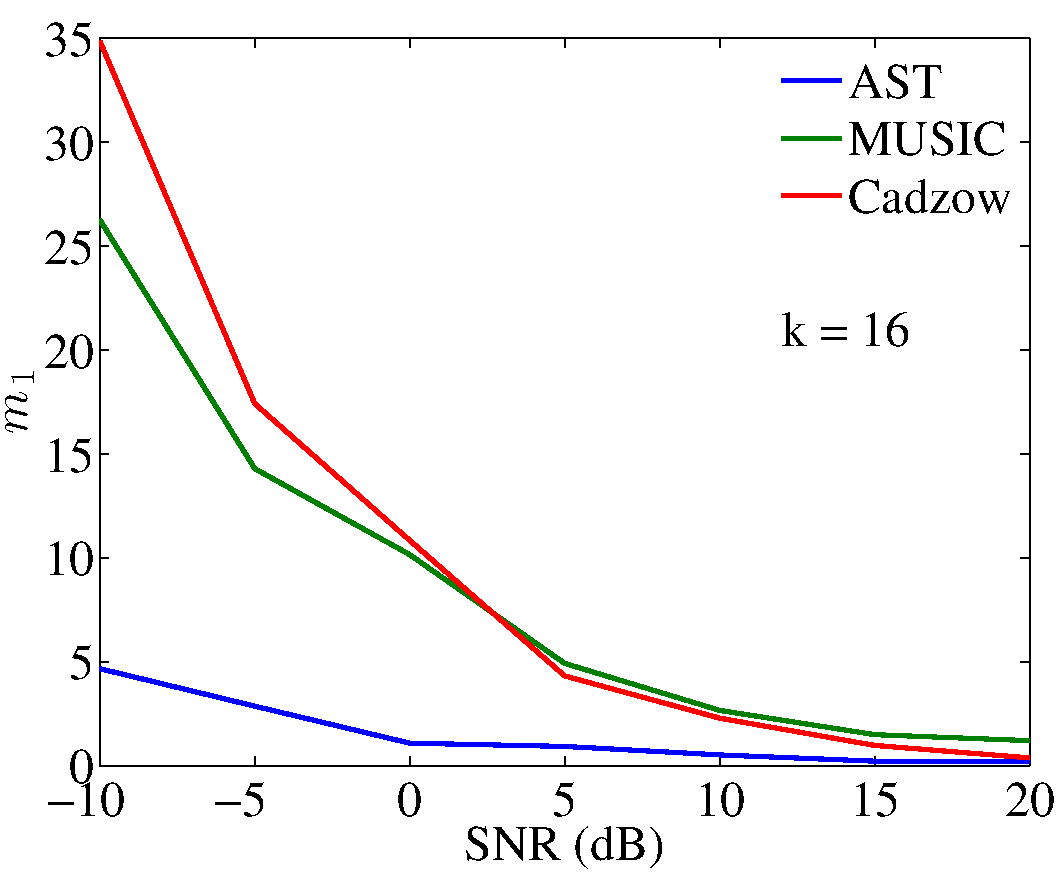
\includegraphics[height=35mm]{figures/mSNR1_16.pdf} &
	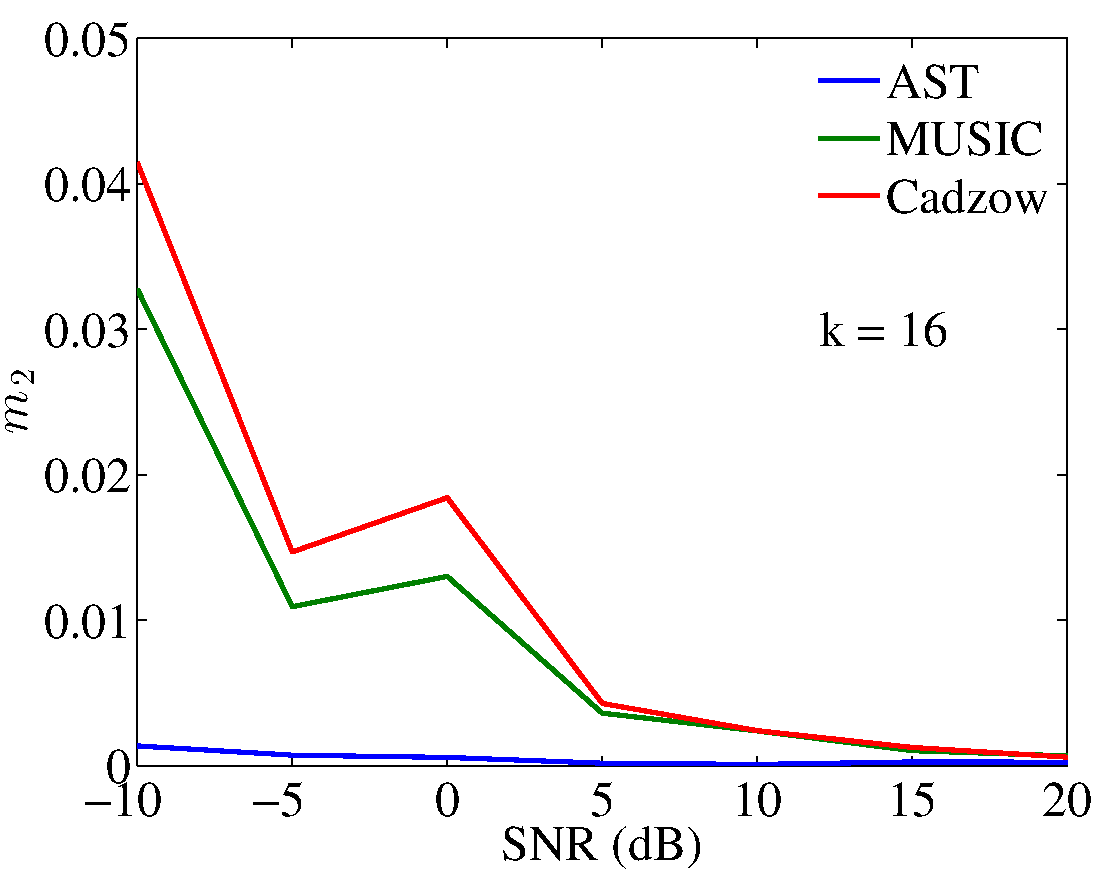
\includegraphics[height=35mm]{figures/mSNR2_16.pdf} &
	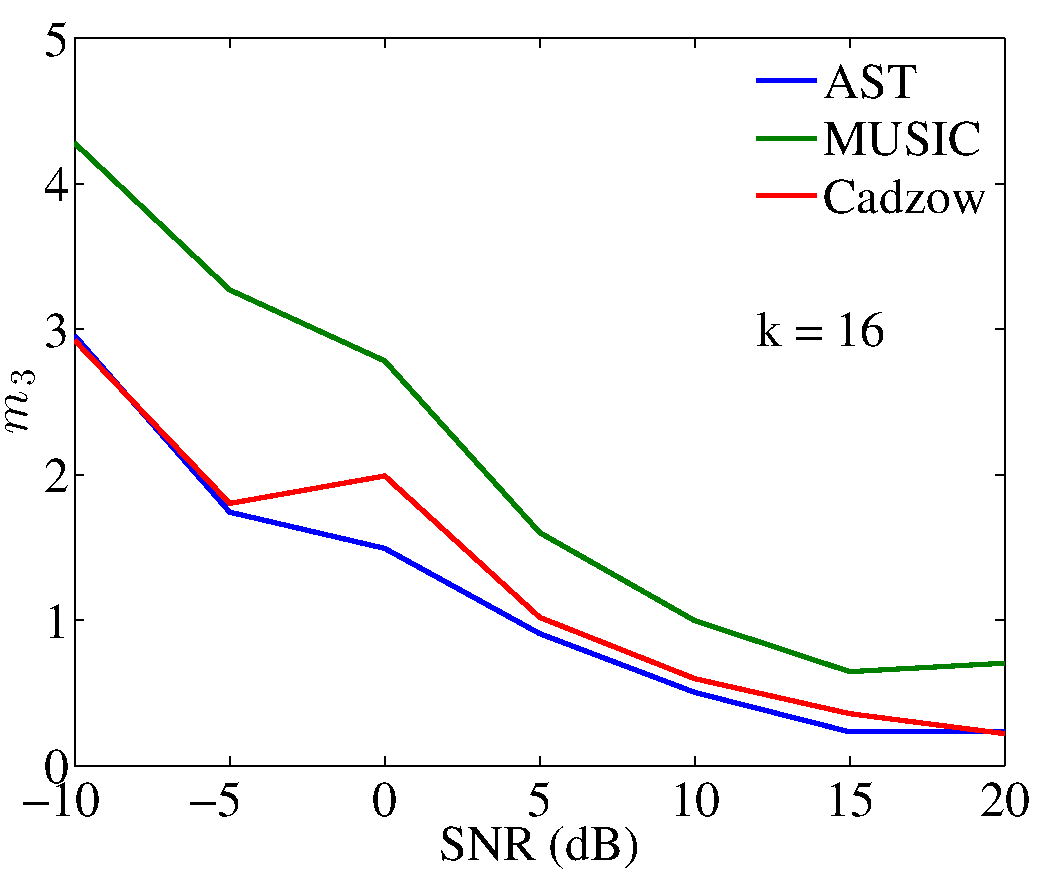
\includegraphics[height=35mm]{figures/mSNR3_16.pdf} \\
	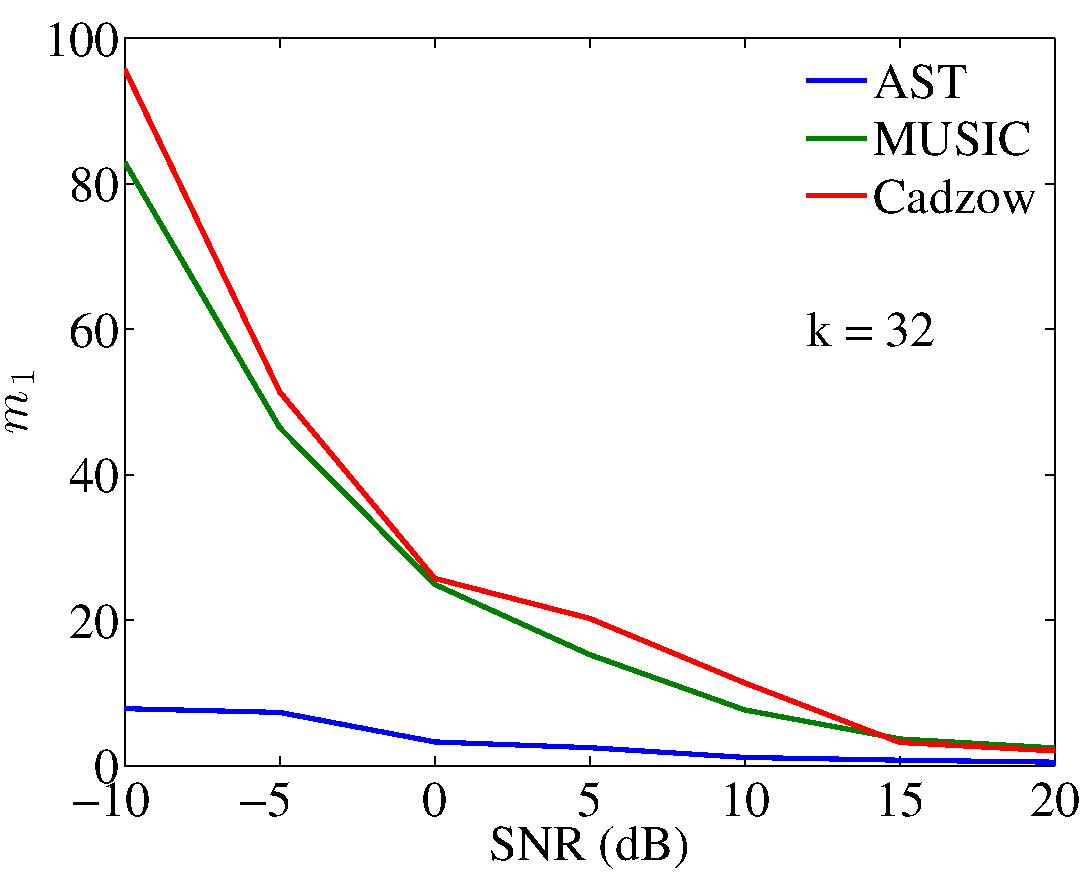
\includegraphics[height=35mm]{figures/mSNR1_32.pdf} &
	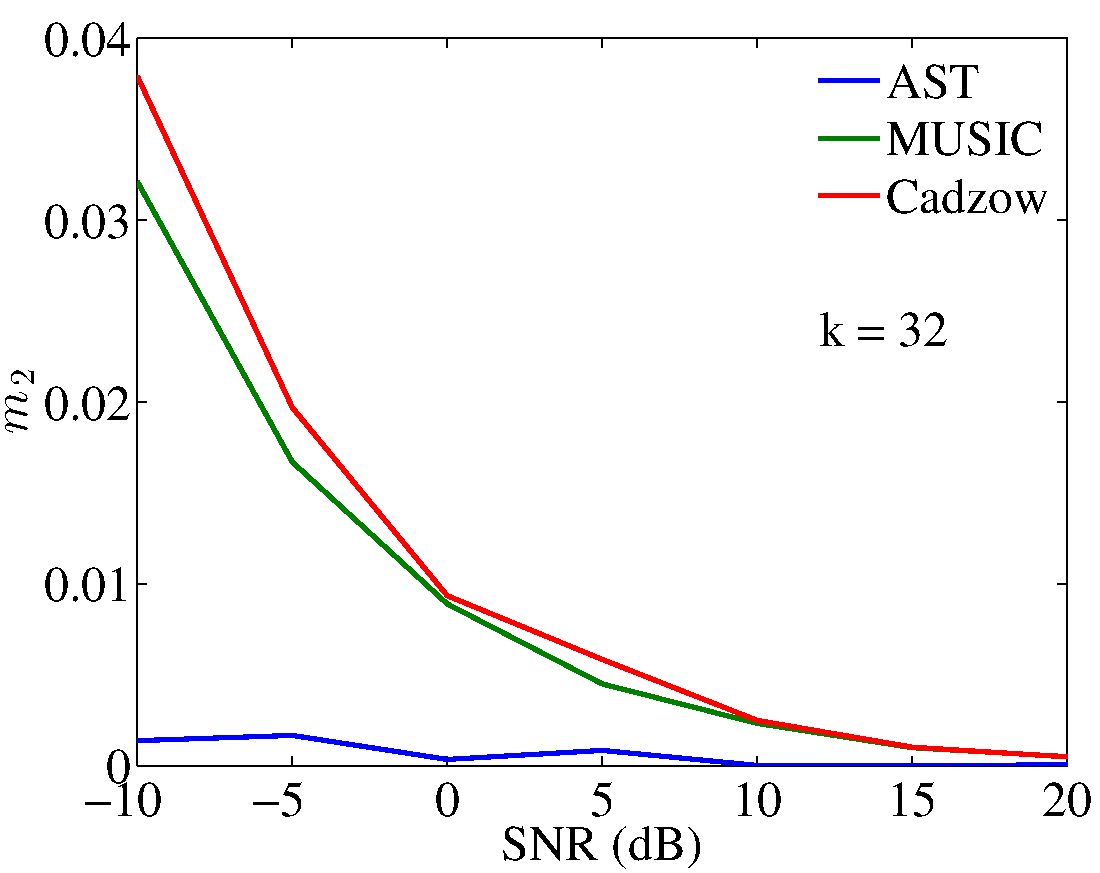
\includegraphics[height=35mm]{figures/mSNR2_32.pdf} &
	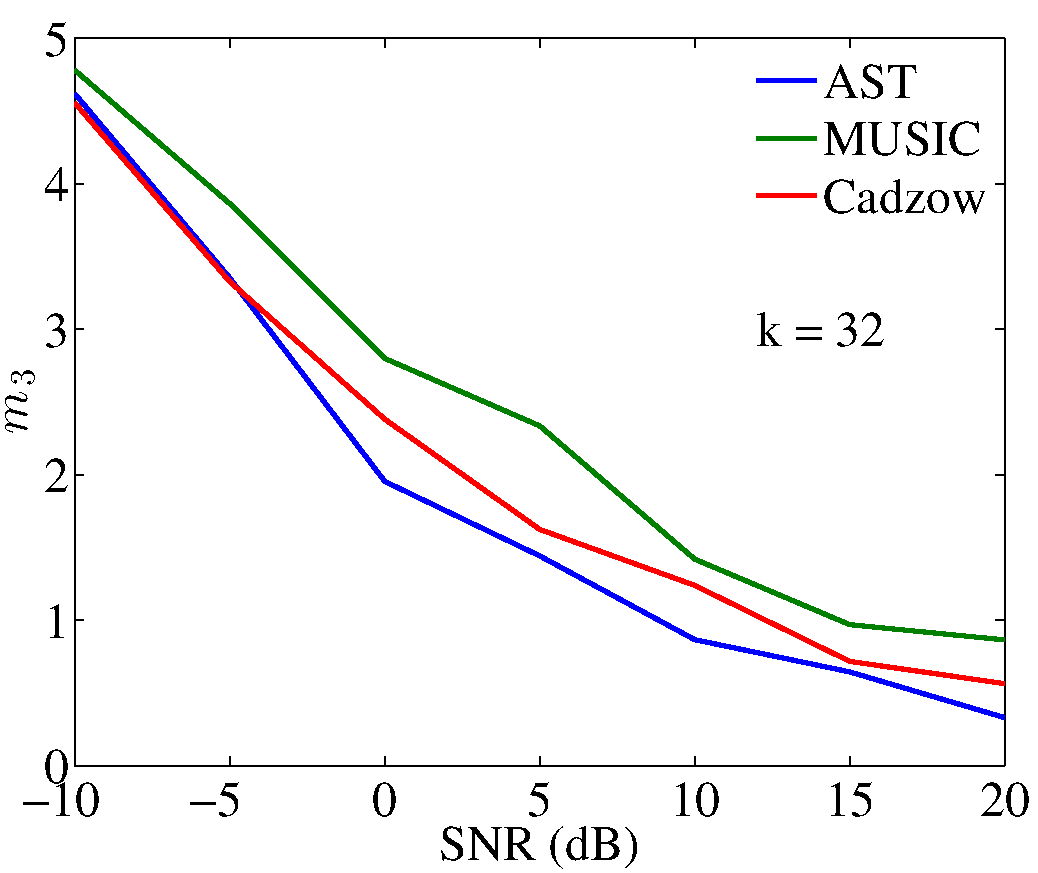
\includegraphics[height=35mm]{figures/mSNR3_32.pdf} \\
	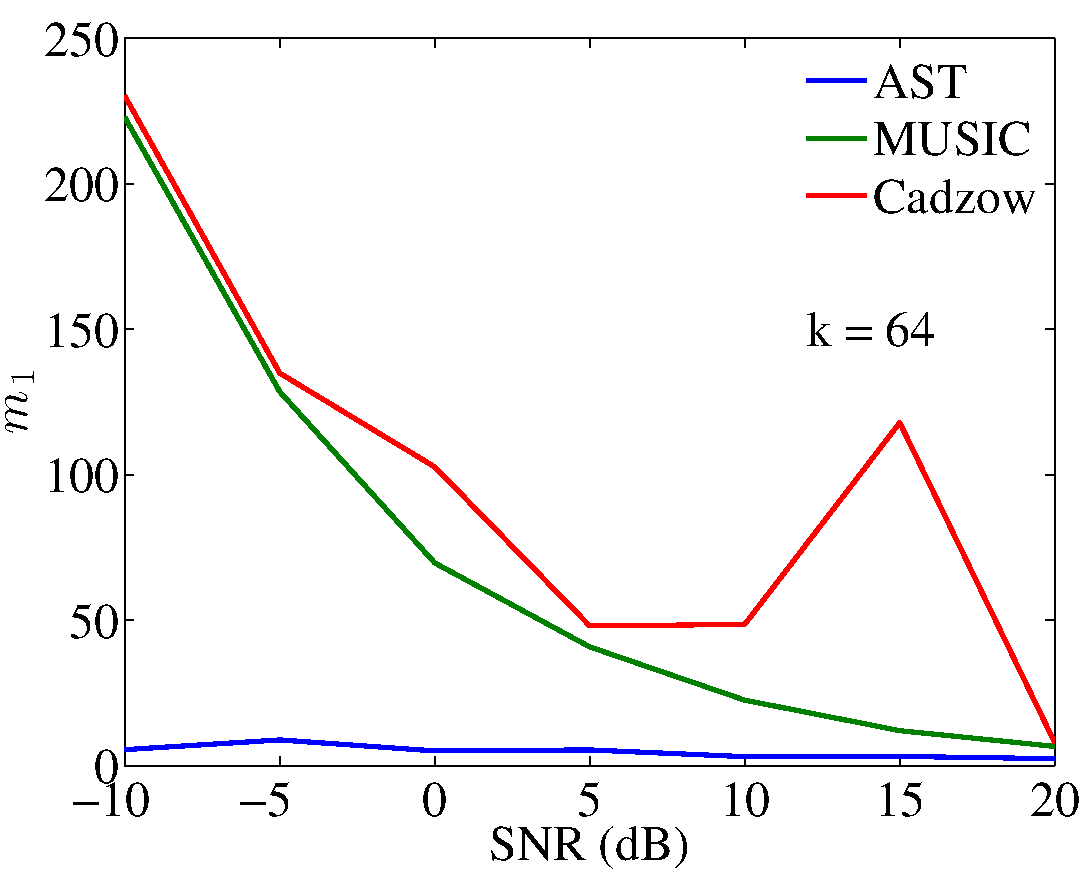
\includegraphics[height=35mm]{figures/mSNR1_64.pdf} &
	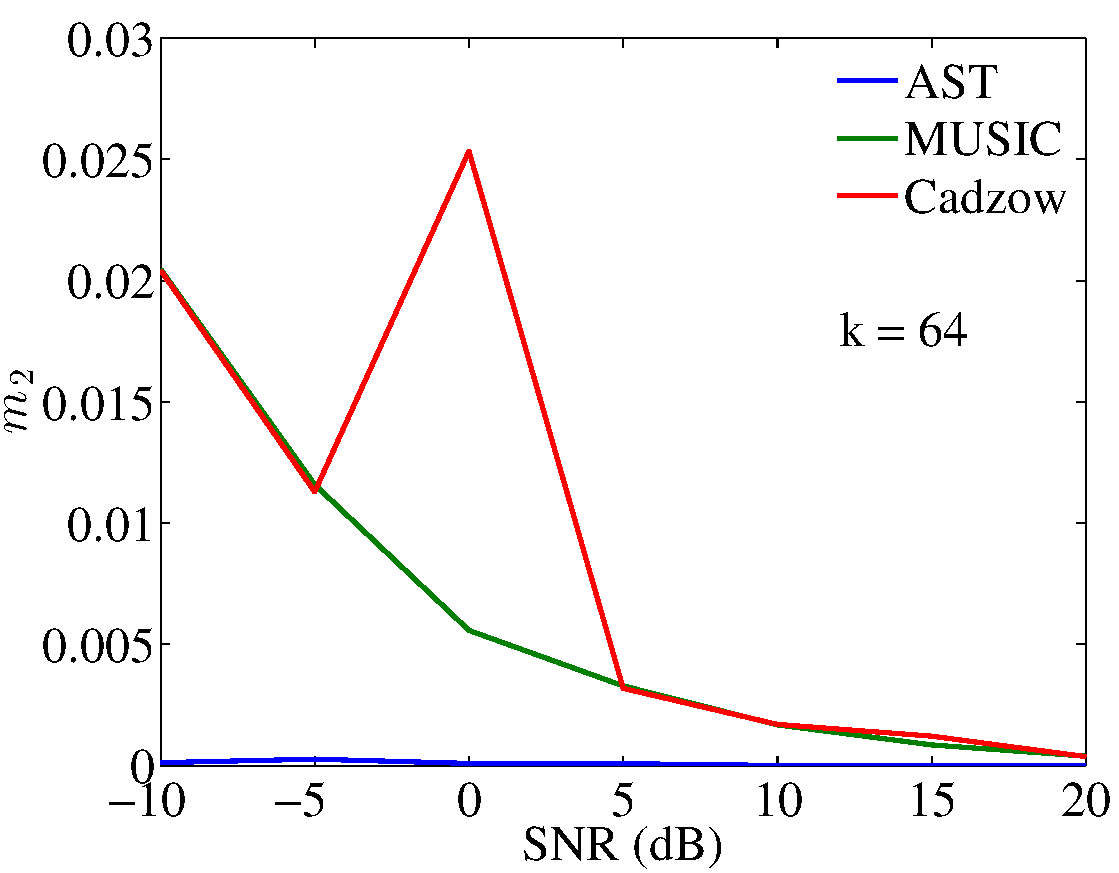
\includegraphics[height=35mm]{figures/mSNR2_64.pdf} &
	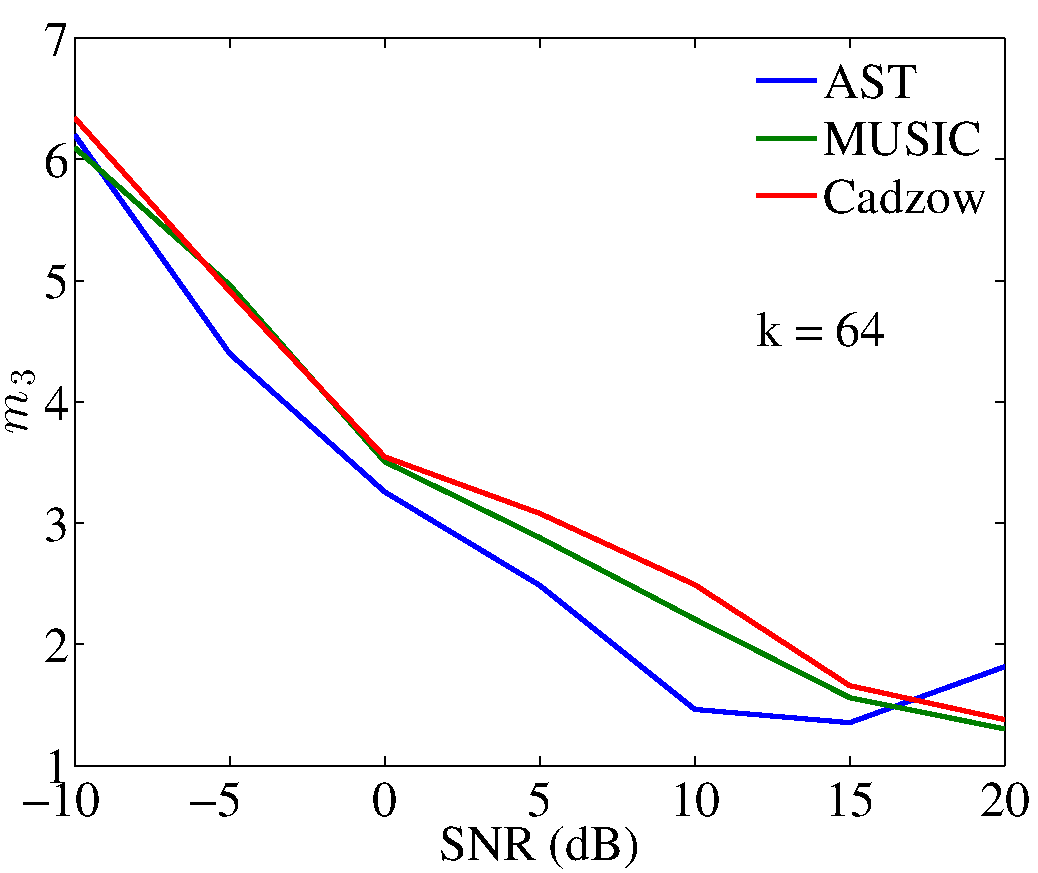
\includegraphics[height=35mm]{figures/mSNR3_64.pdf}
\end{tabular}
\caption{For $n = 256$ samples, the plots from left to right in order measure the average value over 20 random experiments for the error metrics $m_1, m_2$ and $m_3$ respectively. The top, middle and the bottom third of the plots respectively represent the subset of the experiments
with the number of frequencies $k=16, 32$ and $64$.}
\label{fig:msnr}
\end{figure}


We use \emph{performance profiles} to summarize the behavior of the various
algorithms across all of the parameter settings. Performance profiles provide a
good visual indicator of the relative performance of many algorithms under a
variety of experimental conditions\cite{dolanmore02}. Let $\mathcal{P}$ be the
set of experiments and let $\mathrm{MSE}_s(p)$ be the MSE of experiment $p \in
\mathcal{P}$ using the algorithm $s$. Then the ordinate $P_s(\beta)$ of the
graph at $\beta$ specifies the fraction of experiments where the ratio of the
MSE of the algorithm $s$ to the minimum MSE across all algorithms for the given
experiment is less than $\beta$, i.e.,

\begin{equation*}
P_s(\beta) = \frac{\mathop{\#}\left\{p \in \mathcal{P} ~:~ \mathrm{MSE}_s(p) \leq \beta \min_s \mathrm{MSE}_s(p)\right\}}{\mathop{\#}(\mathcal{P})}
\end{equation*}

\begin{figure}[htp]
\centering
\begin{tabular}{cc}
	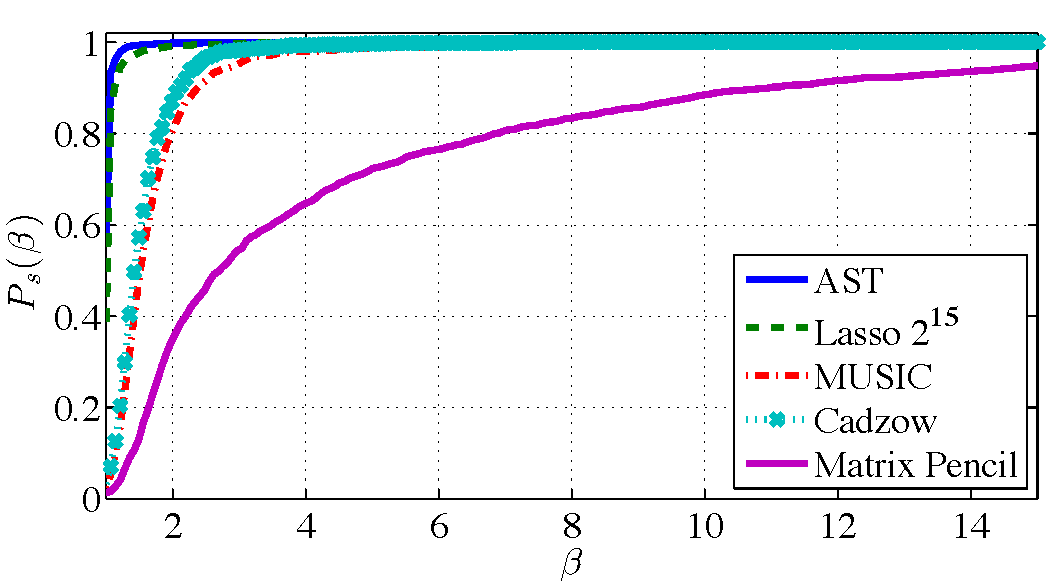
\includegraphics[height=40mm]{figures/performance_profile_randamp_color} &
	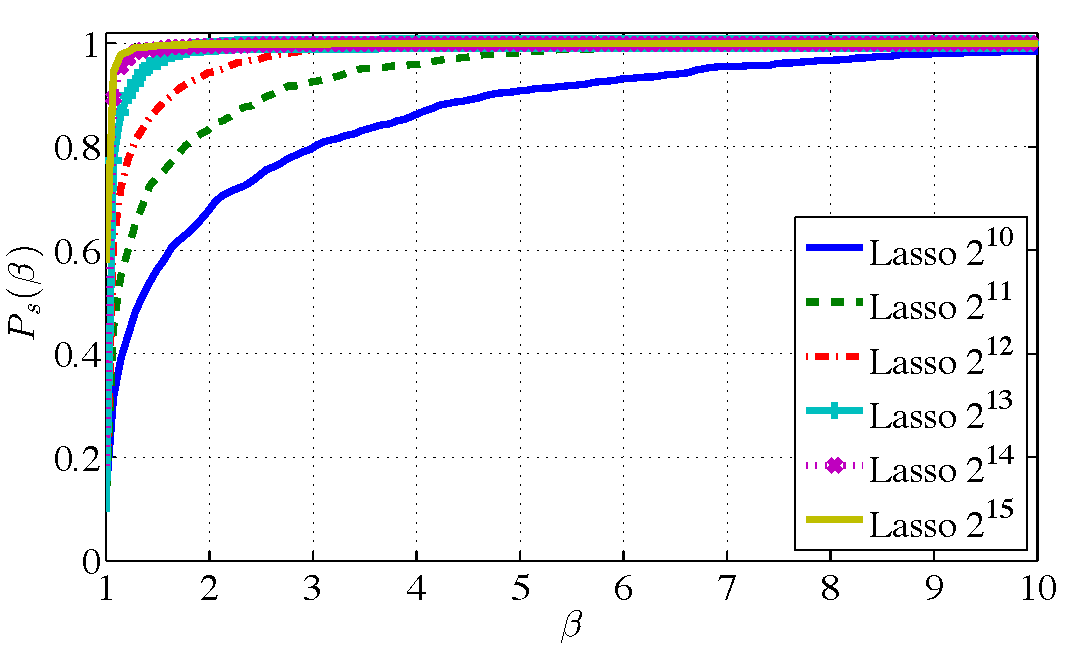
\includegraphics[trim=0mm 0mm 2mm 5mm,clip,height=40mm]{figures/performance_profile_lasso_randamp_color}\\
(a) & (b)
\end{tabular}
\caption{ (a) Performance Profile  comparing various algorithms and AST. (b) Performance profiles for Lasso with different grid sizes.}
\label{fig:pp1}
\end{figure}


From the performance profile in Figure~\ref{fig:pp1}(a), we see that AST is the
best performing algorithm, with Lasso coming in
second. Cadzow does not perform as well as AST, even though it is fed the true
number of sinusoids. When Cadzow is fed an incorrect $k$, even off by $1$, the
performance degrades drastically, and never provides adequate mean-squared
error. Figure~\ref{fig:pp1}(b) shows that the denoising performance
improves  with grid size.

\begin{figure}[htp]
\begin{tabular}{ccc}
	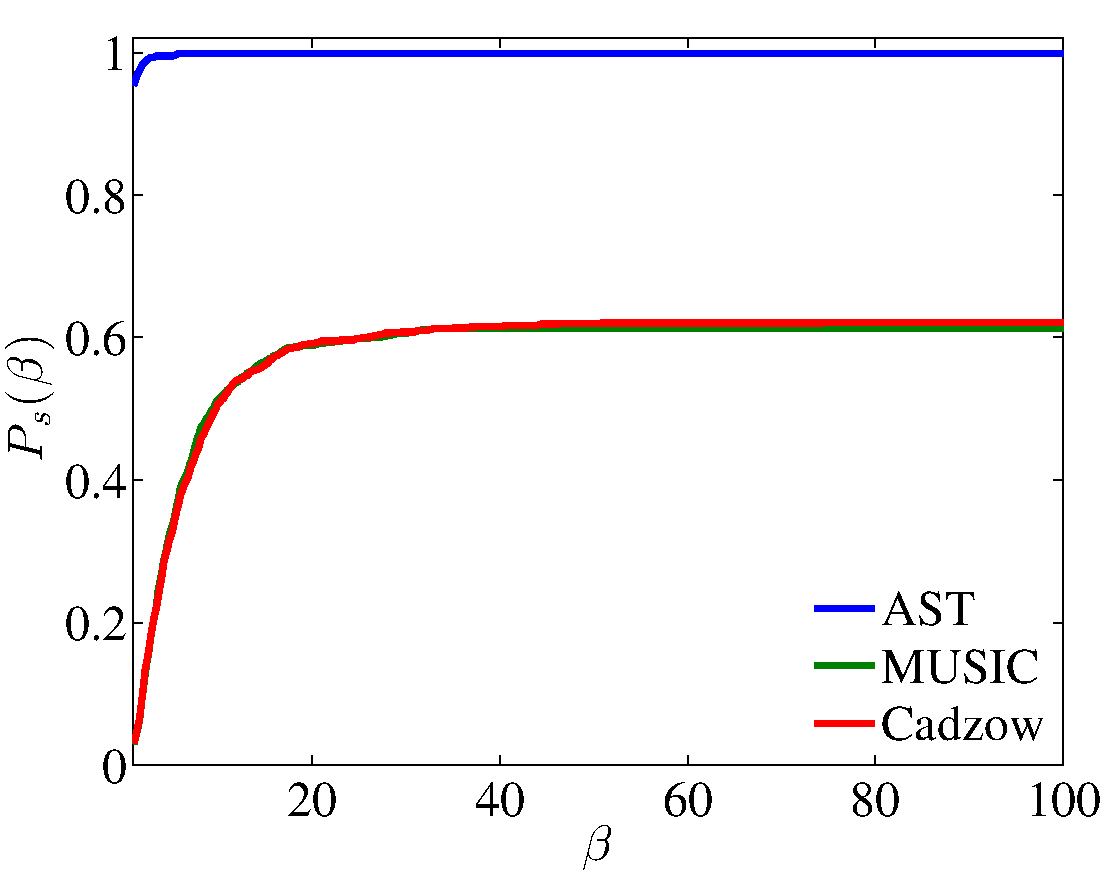
\includegraphics[height=35mm]{figures/m1_pp.pdf} &
	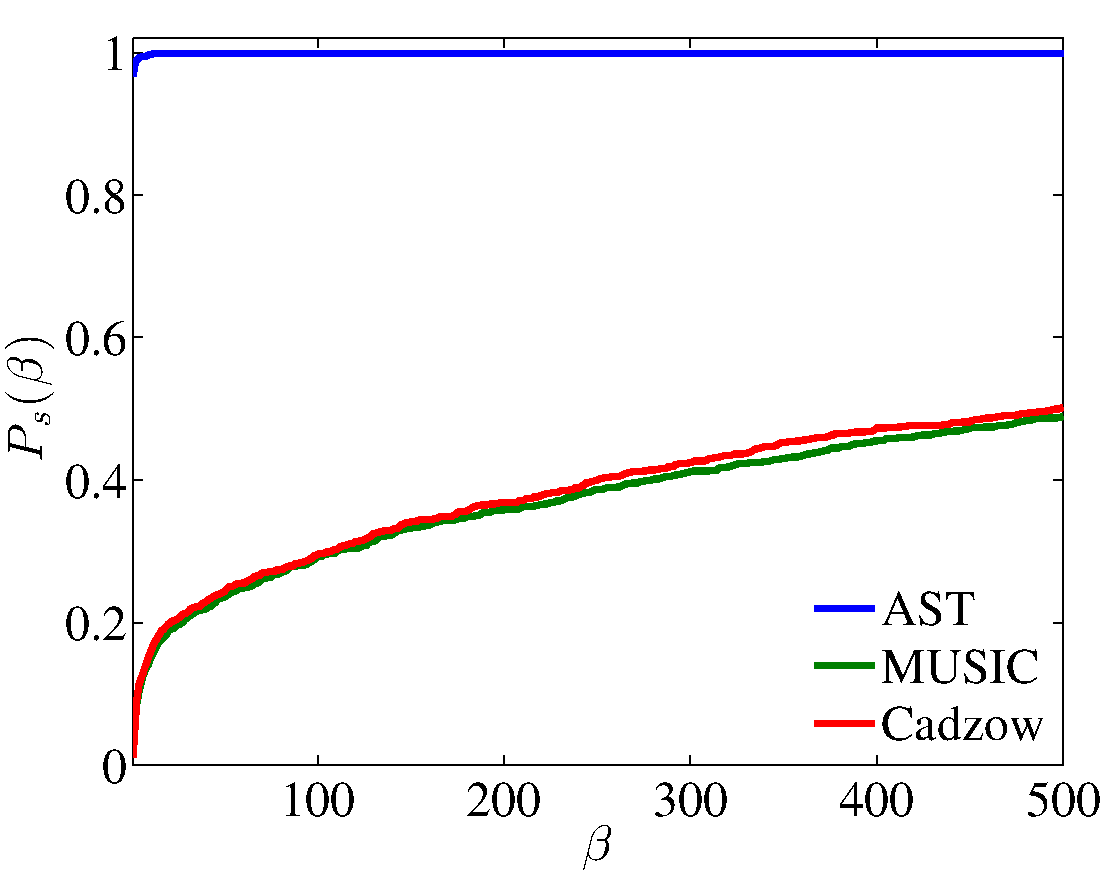
\includegraphics[height=35mm]{figures/m2_pp.pdf} &
	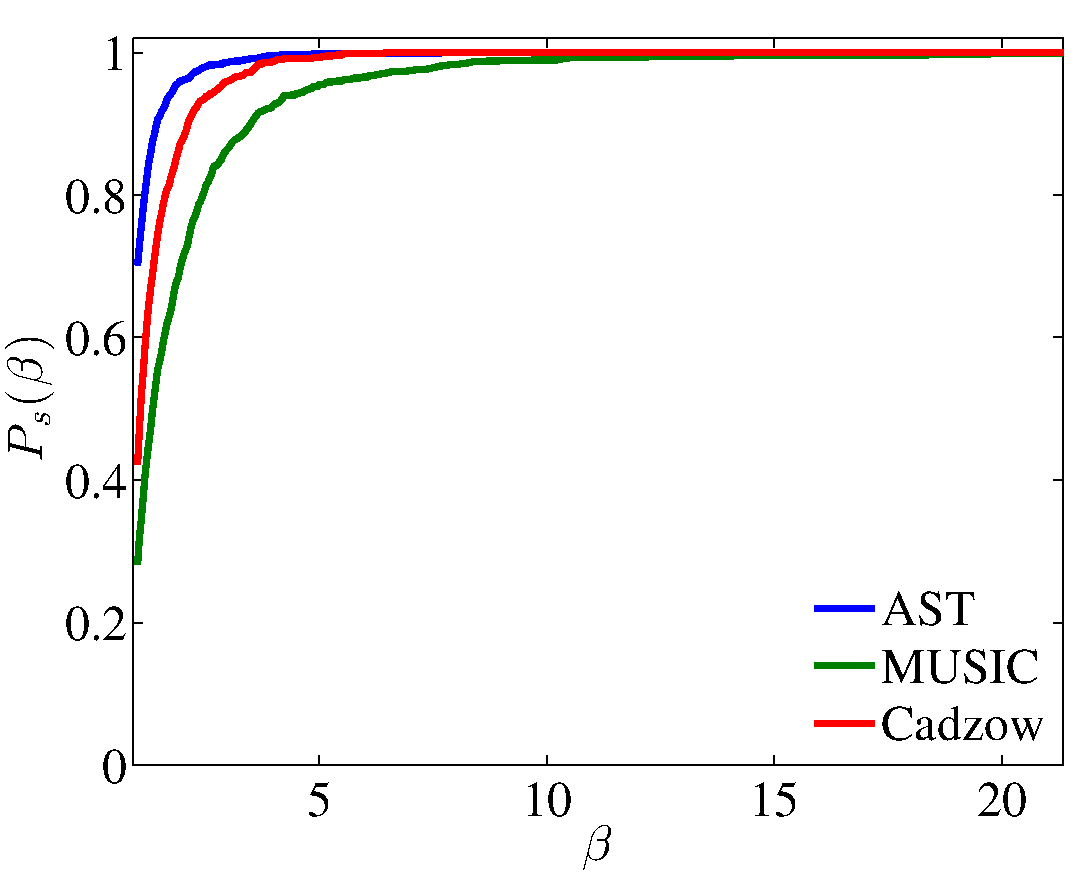
\includegraphics[height=35mm]{figures/m3_pp.pdf}\\
	(a) $m_1$ & (b) $m_2$ & (c) $m_3$
\end{tabular}
\caption{ Performance Profiles for AST, MUSIC and Cadzow.
(a) Sum of the absolute value of amplitudes in the far region ($m_1$)
(b) The weighted frequency localization error, $m_2$
(c) Error in approximation of amplitudes in the near region, $m_3$ }
\label{fig:pp2}
\end{figure}

The performance profiles in Figure~\ref{fig:pp2} show that AST is the best
performing algorithm for all the three metrics for frequency localization. AST
in fact outperforms MUSIC and Cadzow by a substantial margin for metrics $m_1$
and $m_2$.


\section{Conclusion and Future Work}\label{sec:conclusions}

The Atomic norm formulation of line spectral estimation provides several
advantages over prior approaches. By performing the analysis in the continuous
domain we were able to derive simple closed form rates using fairly
straightforward techniques. We only grid the unit circle at the very end of our
analysis and determine the loss incurred from discretization. This approach
allowed us to circumvent some of the more complicated theoretical arguments that
arise when using concepts from compressed sensing or random matrix theory.

In this paper, we demonstrated stability of atomic norm regularization by
analysis of specific properties of the atomic set of moments and the associated
dual space of trigonometric polynomials. The key to our analysis is the
existence and properties of various trigonometric polynomials associated with
signals with well separated frequencies. This work provides several interesting
possible future directions, both in line spectral estimation and in signal
processing in general. We conclude with a short outline of some of the
possibilities.

Though we have made significant progress at understanding the theoretical
limits of line-spectral estimation and superresolution, our bounds could still
be improved. For instance, it remains open as to whether the logarithmic term
in Theorem~\ref{main} can be improved to $\log(n/k)$. Deriving such an upper
bound or improving our minimax lower bound would provide an interesting
direction for future work.

Additionally, it is not clear if our localization bounds in
Theorem~\ref{support} have the optimal dependence on the number of sinusoids
$k$. For instance, we expect that the condition on signal amplitudes for
approximate support recovery should not depend on $k$, by comparison with
similar guarantees that have been established for Lasso~\cite{coherence}. We
additionally conjecture that for a large enough regularization parameter, there
will be no spurious recovered frequencies in the solution. That is, there
should be no non-zero coefficients in the ``far region'' $F$ in
Theorem~\ref{support}. Future work should investigate whether better guarantees
on frequency localization are possible.

% Our work also naturally extends to moment problems where the atomic measures are
% supported on the unit disk in the complex plane. These problems arise naturally
% in controls and systems theory and include model order reduction, system
% identification, and control design. Applying the standard program developed in
% Section~\ref{sec:abstract-denoising} provides a new look at these classic
% operator theory problems in control theory. It would be of significant
% importance to develop specialized atomic-norm denoising algorithms for control
% theoretic problems. Such an approach could yield novel statistical bounds for
% estimation of rational functions and $\mathcal{H}_\infty$-norm approximations.

\begin{subappendices} % (fold)
	
\section{Appendix}
\label{apx:collection}

In this section, we collect useful results from previous work which we use in
our analysis. In addition to Theorem~\ref{dual-stab}, we recall another result
in~\cite{cg_noisy} where the authors show the existence of a trigonometric
polynomial $Q_1$ that is linear in each $N_j$ which is also an essential
ingredient in our proof.

\begin{theorem}[Lemma 2.7 in~\cite{cg_noisy}]
\label{dual-lin}
For any $f_1, \ldots, f_k$ satisfying \eqref{min-sep} and any sign vector $v \in \C^k$ with $|v_j|=1$, there exists a polynomial $Q_1 = \left<q_1, a(f)\right>$ for some $q_1 \in \C^n$ with the following properties: 
\begin{enumerate}
\item For every $f \in N_j,$ there exists a numerical constant $C_a^1$ such that
\begin{equation}
\label{ca1}
|Q_1(f) - v_j(f-f_j)| \leq \frac{n}{2} C_a^1 (f-f_j)^2
\end{equation}
\item For $f \in F$, there exists a numerical constant $C_b^1$ such that
\begin{equation}
\label{cb1}
|Q_1(f)| \leq \frac{C_b^1}{n}.
\end{equation}
\end{enumerate}
\end{theorem}

We will also need the following straightforward consequence of the constructions of the polynomials in Theorem \ref{dual-stab}, Theorem \ref{dual-lin}, and Section \ref{sec:support}.
\begin{lemma}
\label{l1}
There exists a numerical constant $C$ such that the constructed $Q(f)$ in Theorem \ref{dual-stab}, $Q_1(f)$ in Theorem \ref{dual-lin}, and $Q_j^\star(f)$ in Section \ref{sec:support} satisfy respectively
\begin{align}
\|Q(f)\|_1 &:= \int_0^1{| Q(f)| df} \leq \frac{C k}{n}\label{QL1}\\
\| Q_1(f)\|_1 &\leq \frac{C k}{n^2}\label{Q1L1}\\
\|Q_j^\star\|_1 & \leq \frac{Ck}{n}\label{QjL1}.
\end{align}
\end{lemma}
\begin{proof}
We will give a detailed proof of \eqref{QL1}, and list the necessary modifications for proving \eqref{Q1L1} and \eqref{QjL1}. The dual polynomial $Q(f)$ constructed in \cite{cg_exact12} is of the
form
\begin{eqnarray}
  Q \left( f \right) & = & \sum_{f_j \in T} \alpha_j K \left( f - f_j \right)
  + \sum_{f_j \in T} \beta_j K' \left( f - f_j \right) \label{formofQ}
\end{eqnarray}
where $K \left( f \right)$ is the squared Fej\'er kernel (recall that $m = (n-1)/2$)
\begin{eqnarray*}
  K \left( f \right) & = & \left( \frac{\sin \left( \left( \frac{m}{2} + 1
  \right) \pi f \right)}{\left( \frac{m}{2} + 1 \right) \sin \left( \pi f
  \right)} \right)^4
\end{eqnarray*}
 and for $n \geq 257$, the coefficients
$\alpha \in \C^k$ and $\beta \in \C^k$ satisfy \cite[Lemma 2.2]{cg_exact12}
\begin{eqnarray*}
  \left\| \alpha \right\|_{\infty} & \leq & C_\alpha\\
  \left\| \beta \right\|_{\infty} & \leq & \frac{C_\beta}{n} 
\end{eqnarray*}
for some numerical constants $C_\alpha$ and $C_\beta$. 
Using \eqref{formofQ} and triangle inequality, we bound $\|Q(f)\|_1$ as follows: 
\begin{eqnarray}
  \|Q(f)\|_1 &=& \int_0^1 \left| Q \left( f \right) \right| d f\nonumber\\
  &\leq & k \left\| \alpha \right\|_\infty \int_0^1 \left| K \left( f\right) \right| d f + k \left\| \beta \right\|_\infty \int_0^1 \left| K' \left( f\right) \right| d f\label{Qbdgeneral1}\\
  & \leq & C_\alpha k \int_0^1 \left| K \left(f\right) \right| d f + \frac{C_\beta}{n} k \int_0^1 \left|K'(f)\right|d f \label{Q1bd},
 \end{eqnarray}
 
To continue, note that $\int_0^1 | K ( f) | d  f = \int_0^1 | G ( f) |^2 d
 f =: \|G(f)\|_2^2$ where $G ( f)$ is the Fej\'er kernel, since $K(f)$ is the squared
Fej\'er kernel. We can write
\begin{eqnarray}
  G ( f)  =  \left( \frac{\sin \left( \pi \left( \frac{m}{2} + 1 \right) f
  \right)}{\left( \frac{m}{2} + 1 \right) \sin ( \pi f)} \right)^2
   =  \sum_{l = - m / 2}^{m / 2} g_l e^{- i 2 \pi f l}\label{expressionG}
\end{eqnarray}
where $g_l = \left( \frac{m}{2} + 1 - | l | \right) / \left( \frac{m}{2} + 1
\right)^2$. Now, by using Parseval's identity, we obtain
\begin{eqnarray}
 \int_0^1 |K(f)| df & = & \int_0^1 | G ( f) |^2 d f
  =  \sum_{l = - m / 2}^{m / 2} | g_l |^2\nonumber\\
  & = & \frac{1}{\left( \frac{m}{2} + 1 \right)^4} \left( \left( \frac{m}{2}
  + 1 \right)^2 + 2 \sum_{l = 1}^{m / 2} \left( \frac{m}{2} + 1 - l \right)^2
  \right)\nonumber\\
  & = & \frac{1}{\left( \frac{m}{2} + 1 \right)^4} \left( \left( \frac{m}{2}
  + 1 \right)^2 + 2 \sum_{l = 1}^{m / 2} l^2 \right)\nonumber\\
  & \leq & \frac{C}{n}\label{bdKf}
\end{eqnarray}
for some numerical constant $C$ when $n = 2 m + 1 \geq 10$.

Now let us turn our attention to $\int_0^1 | K' (
f) | d  f$. Since $K ( f) = G ( f)^2$, we have
\begin{eqnarray}
  \int_0^1 | K' ( f) | d  f  =  2\int_0^1 | G ( f) G' ( f) | d
   f
   \leq  2\| G ( f) \|_2 \| G' ( f) \|_2\label{eq:holder-int}
\end{eqnarray}
We have already established that $\| G ( f) \|_2^2 \leq C / {n}$ and we
will now show that $\| G' ( f) \|_2^2 \leq C' {n}$. Differentiating the
expression for $G(f)$ in \eqref{expressionG}, we get
\begin{eqnarray*}
  G' ( f) & = & -2 \pi i \sum_{l = - m / 2}^{m / 2} l g_l e^{- i 2 \pi f l}
\end{eqnarray*}
Therefore, by applying Parseval's identity again, we get
\begin{eqnarray*}
  \| G' ( f) \|_2^2 
  & = & 4 \pi^2 \sum_{l = - m / 2}^{m / 2} l^2 | g_l |^2\\
  & \leq &  \pi^2 m^2 \sum_{l = - m / 2}^{m / 2} | g_l |^2\\
  & \leq & C' n
\end{eqnarray*}
Plugging back into \eqref{eq:holder-int} yields
\begin{align}
\int_0^1 |K'(f)| df \leq C \label{bdK1f}
\end{align}
for some constant $C$. Combining \eqref{bdK1f} and \eqref{bdKf} with \eqref{Q1bd} gives the desired result in \eqref{QL1}.



The dual polynomial $Q_1(f)$ is also of the form \eqref{formofQ} with coefficient vectors $\alpha_1$ and $\beta_1$, which satisfy \cite[Proof of Lemma 2.7]{cg_noisy}
\begin{align*}
\|\alpha_1\|_\infty \leq \frac{C_{\alpha_1}}{n},\\
\|\beta_1\|_\infty \leq \frac{C_{\beta_1}}{n^2}.
\end{align*}
Combining the above two bounds with \eqref{Qbdgeneral1}, \eqref{bdK1f} and \eqref{bdKf} gives the desired result in \eqref{Q1L1}.

The last polynomial $Q_j^\star$ also has the form \eqref{formofQ} with coefficient vectors $\alpha^\star$ and $\beta^\star$. According to \cite[Proof of Lemma 2.2]{granda2}, these coefficients satisfy
\begin{align*}
\|\alpha^\star\|_\infty \leq {C_{\alpha_\star}},\\
\|\beta_\star\|_\infty \leq \frac{C_{\beta_\star}}{n},
\end{align*}
which yields \eqref{QjL1} following the same argument leading to \eqref{QL1}. 

\end{proof}

Using Lemma \ref{l1}, we can derive the estimates we need in the following lemma.
\begin{lemma}
\label{l4}
Let $\nu = \hat{\mu} - \mu$ be the difference measure. Then, there exists numerical constant $C>0$ such that
\begin{align}
\label{qv}\left| \int_0^1 Q(f) \nu(df) \right| &\leq \frac{C k \tau}{n}\\
\label{q1v}\left| \int_0^1 Q_1(f) \nu(df) \right| &\leq \frac{C k \tau}{n^2}\\
\label{qjv} \left| \int_0^1 Q_j^\star(f) \nu(df) \right| & \leq \frac{Ck\tau}{n}.
\end{align}
\end{lemma}
\begin{proof}
Let $Q_0 = \langle q_0, a(f) \rangle $ be a general trigonometric polynomial associated with $q_0 \in \C^n$. Then,
\begin{align*}
\left|\int_0^1 Q_0(f) \nu(df) \right| 
& = \left|\int_0^1 \langle q_0 , a(f) \rangle  \nu(df) \right|\\
& = \left|\langle q_0,  \int_0^1  a(f)  \nu(df) \rangle\right|\\
& = \left|\langle q_0, e \rangle\right|\\
& = \left|\langle Q_0(f), E(f) \rangle\right|\\
& \leq \vnorm{Q_0(f)}_1 \vnorm{E(f)}_\infty\,.
\end{align*}
Here we use Parseval's identity in the second to last step and H\"{o}lder's inequality in the last inequality. Then, the result follows by using Lemma~\ref{l1} and \eqref{errbd}.
\end{proof}


We also need the following consequence of the optimality condition of AST from~\cite[Lemma 2]{btr12}:
\begin{prop}\label{pro:optimality}
\begin{align}
\tau \vnorm{\hat{x}}_\A \leq \tau \vnorm{x^\star}_\A + \langle w, \hat{x} - x^\star \rangle
\end{align}
\end{prop}


\end{subappendices}
